% lsqvce -- Theory, practice, implementation, error handling, and the R5
% review and redesign plan.  Built with pdflatex (dev/docs_src/theory_r5/build.sh).
% Created 2026-09-01 (CEST, UTC+02:00) with assistance from Claude (Anthropic),
% model Claude Fable 5.1 -- REVIEW R5.
\documentclass[11pt,a4paper,twoside,openany]{report}
\usepackage[T1]{fontenc}
\usepackage[utf8]{inputenc}
\usepackage{mathptmx}\usepackage[scaled=0.92]{helvet}\usepackage{courier}
\usepackage{microtype}
\usepackage[margin=24mm,headheight=14pt]{geometry}
\usepackage{amsmath,amssymb,bm}
\usepackage{booktabs,longtable,array,multirow}
\usepackage{xcolor}
\usepackage{enumitem}
\usepackage{listings}
\usepackage{tikz}
\usetikzlibrary{arrows.meta,positioning,shapes.geometric,fit,calc}
\usepackage[most]{tcolorbox}
\usepackage{titlesec}
\usepackage{caption}
\usepackage{fancyhdr}
\usepackage[hidelinks,pdftitle={lsqvce -- Theory, practice, implementation, error handling; R5 review and redesign},pdfauthor={Matthias Weigelt with Claude (Anthropic), model Claude Fable 5.1}]{hyperref}

\setlist{nosep,leftmargin=*}
\setlength{\tabcolsep}{4pt}
\newcolumntype{P}[1]{>{\raggedright\arraybackslash}p{#1}}
\sloppy
\setlength{\parskip}{4pt}
\setlength{\parindent}{0pt}
\titleformat{\chapter}[hang]{\bfseries\LARGE}{\thechapter}{1em}{}
\titlespacing*{\chapter}{0pt}{-10pt}{14pt}
\titleformat{\part}[display]{\bfseries\huge}{Part \thepart}{1em}{}

\definecolor{ink}{RGB}{30,30,30}
\definecolor{rule}{RGB}{120,120,120}
\definecolor{boxbg}{RGB}{245,245,240}
\definecolor{warnbg}{RGB}{253,244,235}
\definecolor{codebg}{RGB}{247,247,247}
\definecolor{kw}{RGB}{0,0,160}
\definecolor{cm}{RGB}{34,120,34}
\definecolor{st}{RGB}{160,32,240}

\lstdefinelanguage{MATLABx}{
  morekeywords={function,end,if,else,elseif,for,while,return,arguments,classdef,properties,methods,switch,case,otherwise,try,catch,parfor,spmd},
  sensitive=true, morecomment=[l]{\%}, morestring=[m]', morestring=[m]"}
\lstset{language=MATLABx,basicstyle=\ttfamily\small,keywordstyle=\color{kw},commentstyle=\color{cm},stringstyle=\color{st},
  backgroundcolor=\color{codebg},frame=single,rulecolor=\color{rule},framesep=4pt,breaklines=true,columns=fullflexible,keepspaces=true,
  showstringspaces=false,aboveskip=6pt,belowskip=6pt,xleftmargin=2pt}

\newtcolorbox{principle}[1][]{enhanced,colback=boxbg,colframe=rule,boxrule=0.5pt,arc=1pt,left=6pt,right=6pt,top=4pt,bottom=4pt,fonttitle=\bfseries,title={#1}}
\newtcolorbox{caveat}[1][]{enhanced,colback=warnbg,colframe=rule,boxrule=0.5pt,arc=1pt,left=6pt,right=6pt,top=4pt,bottom=4pt,fonttitle=\bfseries,title={#1}}
\newtcolorbox{panel}[1][]{enhanced,colback=white,colframe=rule,boxrule=0.5pt,arc=1pt,left=6pt,right=6pt,top=4pt,bottom=4pt,fonttitle=\bfseries,title={#1},breakable}

\newcommand{\mat}[1]{\bm{#1}}
\newcommand{\vc}[1]{\bm{#1}}
\newcommand{\T}{^{\mathsf T}}
\newcommand{\tr}{\operatorname{tr}}
\newcommand{\diag}{\operatorname{diag}}
\newcommand{\E}{\operatorname{E}}
\newcommand{\Var}{\operatorname{Var}}
\newcommand{\code}[1]{\texttt{#1}}
\newcommand{\lsq}{\code{lsqvce}}
\newcommand{\finding}[1]{\textbf{#1}}

\pagestyle{fancy}
\fancyhf{}
\fancyhead[LE,RO]{\small\thepage}
\fancyhead[RE]{\small\nouppercase{\leftmark}}
\fancyhead[LO]{\small lsqvce -- theory, practice, implementation, error handling; R5 review and redesign}
\renewcommand{\headrulewidth}{0.3pt}

\begin{document}

\begin{titlepage}
\vspace*{30mm}
{\bfseries\Huge lsqvce\par}
\vspace{6mm}
{\bfseries\LARGE Least-squares adjustment with variance component estimation\par}
\vspace{4mm}
{\Large Theory, practical considerations, implementation, and error handling\par}
\vspace{2mm}
{\Large --- with the Review R5 of toolbox v4.0 and the redesign plan for v5\par}
\vspace{14mm}
{\large Prepared for the \lsq{} toolbox (\code{matweigelt/lsqvce}) by a three-expert panel:\par}
\vspace{3mm}
\begin{tabular}{@{}ll@{}}
Expert A & least-squares adjustment and stochastic error modelling\\
Expert B & satellite-gravimetry data processing (GRACE/GRACE-FO)\\
Expert C & software design and MATLAB programming\\
\end{tabular}
\vspace{14mm}

{\large Version 5.0-plan, 1 September 2026 --- the R5 record; implementation authority: the Manual\par}
\vspace{3mm}
{Created 2026-09-01 (CEST, UTC+02:00) with assistance from Claude (Anthropic), model Claude Fable 5.1 --- Review R5. Source: \code{dev/docs\_src/theory\_r5/}. Binding status and ledger: \code{dev/HANDOVER.md} \S12.\par}
\vfill
\begin{principle}[How to read this document]
Parts I--III are the \emph{theory authority} of the toolbox: what is computed, why, and where the computation must refuse. They supersede \code{lsqvce\_theory.pdf} (R4 WP-59) once decision R5-D6 is taken. Parts IV--V are the review of the tree at \code{main} head \code{d7ad051} (v4.0, 634 test points, 83 public names) and the plan for v5. Every claim about the toolbox names a file, a line or a work package so it can be checked rather than believed. Nothing in Part V is implemented; it is a plan awaiting the user's decisions (\S\ref{sec:decisions}).
\end{principle}
\begin{principle}[Where this record stops (added 2026-09-09, R6 WP-106)]
Parts IV--V and Appendix C are a DATED RECORD: the review of v4.0 and the plan and option mapping of v5.0 as of 1--3 September 2026. They are kept as written. Every implementation-facing statement in them --- the \code{epochCovariance} hook, \code{arcId}, the \code{lsqvce:fit:notYet} refusal of a robust pass on the streaming kind, \code{LogFile}, the 14-knob option table --- has since been superseded, and the current state is NOT in this document: the \emph{implementation authority} is the Manual (\code{doc lsqvce}, chapters 3, 4 and 7), \code{RELEASE\_NOTES.md} lists what changed per version (5.1 \ldots{} 6.1), and \code{dev/HANDOVER.md} \S12 carries the decisions. Parts I--III (the theory) are current.
\end{principle}
\end{titlepage}

\tableofcontents

\part{Theory}

\chapter{The linear model and its solutions}
\label{ch:model}

\section{Gauss--Markov model}

The toolbox estimates $u$ unknowns $\vc{x}$ from $n$ \emph{reduced} observations $\vc{l}$ (observed minus computed at the linearisation point) under the linear Gauss--Markov model
\begin{equation}
\vc{l} = \mat{A}\vc{x} + \vc{e}, \qquad \E[\vc{e}] = \vc{0}, \qquad \E[\vc{e}\vc{e}\T] = \mat{\Sigma} = \sigma_0^2\,\mat{Q}, \qquad \mat{P} = \mat{Q}^{-1}.
\label{eq:gm}
\end{equation}
$\mat{Q}$ is the a-priori cofactor matrix, $\sigma_0^2$ the variance of unit weight. The best linear unbiased estimate minimises $\vc{e}\T\mat{P}\vc{e}$:
\begin{equation}
\hat{\vc{x}} = (\mat{A}\T\mat{P}\mat{A})^{-1}\mat{A}\T\mat{P}\vc{l} = \mat{N}^{-1}\vc{n}, \qquad
\hat{\vc{v}} = \vc{l} - \mat{A}\hat{\vc{x}}, \qquad
\hat\sigma_0^2 = \frac{\hat{\vc{v}}\T\mat{P}\hat{\vc{v}}}{n-u}, \qquad
\mat{\Sigma}_{\hat x\hat x} = \hat\sigma_0^2\,\mat{N}^{-1}.
\label{eq:lsq}
\end{equation}
Two facts used everywhere below: the residual is a projection, $\hat{\vc{v}} = (\mat{I}-\mat{A}\mat{N}^{-1}\mat{A}\T\mat{P})\,\vc{l} = (\mat{I}-\mat{H})\,\vc{l}$ with the \emph{hat matrix} $\mat{H}$; and the redundancy is distributed over the observations by the diagonal of $\mat{R} = \mat{I}-\mat{H}$, $\sum_i r_i = n-u$ (Förstner 1979). $\hat\sigma_0^2$ is unbiased only because the denominator is that trace: every estimator in Chapter~\ref{ch:vce} is a specialisation of ``quadratic form over its expectation''.

\section{Decorrelation and whitening}

With $\mat{\Sigma} = \mat{W}\T\mat{W}$ (any square root; Cholesky $\mat{W}$ upper triangular, or a filter), the model is transformed to unit weights,
\begin{equation}
\bar{\mat{A}} = \mat{W}^{-\mathsf T}\mat{A}, \qquad \bar{\vc{l}} = \mat{W}^{-\mathsf T}\vc{l}, \qquad \bar{\vc{e}} \sim (\vc{0}, \mat{I}),
\label{eq:whiten}
\end{equation}
and \eqref{eq:lsq} becomes ordinary least squares. The toolbox never forms $\mat{\Sigma}$ or $\mat{P}$ of size $n$: whitening is applied \emph{per arc} by a triangular solve (Toeplitz Cholesky) or by a linear filter (AR/ARMA), Chapter~\ref{ch:stochastic}. Everything downstream --- normal equations, residuals, redundancies --- is expressed in whitened quantities, so ``residual'' in this document means $\bar{\vc{v}} = \mat{W}^{-\mathsf T}\hat{\vc{v}}$ unless said otherwise. The raw residual is recovered as $\hat{\vc{v}} = \mat{W}\T\bar{\vc{v}}$ when a user asks for it.

\section{Two ways to solve, and why the toolbox keeps both}
\label{sec:twosolvers}

\paragraph{Normal equations (NEQ).} Accumulate $\mat{N} = \sum_k \bar{\mat{A}}_k\T\bar{\mat{A}}_k$, $\vc{n} = \sum_k\bar{\mat{A}}_k\T\bar{\vc{l}}_k$ and $\bar{\vc{l}}\T\bar{\vc{l}}$ over arcs $k$, then $\mat{N} = \mat{U}\T\mat{U}$ (Cholesky) and two triangular solves. Cost $O(n u^2 + u^3/3)$, memory $O(u^2)$, and --- decisive in satellite geodesy --- \emph{partial systems add}: arcs, days, satellites, and archived normal equations (SINEX/GROOPS) combine by matrix addition. The price is conditioning: $\kappa(\mat{N}) = \kappa(\bar{\mat{A}})^2$, so $\hat\sigma_0^2$ computed as $(\bar{\vc l}\T\bar{\vc l} - \vc{n}\T\hat{\vc x})/(n-u)$ cancels catastrophically when the fit is very good relative to $\|\vc l\|$ (\S\ref{sec:cancellation}).

\paragraph{Square-root information (QR).} Maintain the triangular factor of $[\bar{\mat{A}}\ \bar{\vc{l}}]$ by Householder updates; $\hat\sigma_0^2$ is the squared last diagonal, obtained \emph{without} subtraction. Backward stable, $\kappa(\bar{\mat A})$ instead of its square; memory the same $O(u^2)$; arcs still add (the factor is updated, not recomputed); but factors of two independent systems do not add --- combination means re-triangularising the stacked factors, which is exact but not the file-exchange convention of the field.

\begin{principle}[Verdict (R4 §11.2 item 2, confirmed by R5)]
NEQ is the default because the block-arrow elimination, day-wise parallel accumulation and NEQ file exchange are NEQ operations; QR is the accuracy fallback. Both stay. The condition evidence ($\kappa$ estimate, pivot ratios) is always reported so a user sees when the default is the wrong choice. What the toolbox must not do is hide the difference by iterative refinement on the NEQ path (``guards are not fixes'', HANDOVER §11.8).
\end{principle}

\section{Block-arrow systems and the elimination of local parameters}
\label{sec:blockarrow}

In satellite gravimetry the unknowns split into \emph{common} parameters $\vc{x}$ (Stokes coefficients, shared by all arcs of all systems) and \emph{local} parameters $\vc{y}_a$ (initial state, accelerometer scale/bias, empirical KBR terms) that appear in one arc, one day or one system only. For system $s$ and arc $a$,
\begin{equation}
\bar{\vc{l}}_a = \bar{\mat{A}}_a\vc{x} + \bar{\mat{B}}_a\vc{y}_a + \bar{\vc{e}}_a ,
\end{equation}
and the joint normal equations have the block-arrow form. Eliminating $\vc{y}_a$ by the Schur complement gives the \emph{reduced} contribution of the arc to the common system:
\begin{equation}
\mat{N}_{a}^{\mathrm{red}} = \bar{\mat{A}}_a\T\bar{\mat{A}}_a - \bar{\mat{A}}_a\T\bar{\mat{B}}_a\,(\bar{\mat{B}}_a\T\bar{\mat{B}}_a)^{-1}\bar{\mat{B}}_a\T\bar{\mat{A}}_a
= \bar{\mat{A}}_a\T\,\mat{P}^{\perp}_{B_a}\,\bar{\mat{A}}_a, \qquad
\vc{n}_a^{\mathrm{red}} = \bar{\mat{A}}_a\T\mat{P}^{\perp}_{B_a}\bar{\vc{l}}_a,
\label{eq:schur}
\end{equation}
with $\mat{P}^{\perp}_{B} = \mat{I} - \bar{\mat{B}}(\bar{\mat{B}}\T\bar{\mat{B}})^{-1}\bar{\mat{B}}\T$ the projector onto the complement of the local design. The residual sum of squares reduces likewise, $\bar{\vc{l}}_a\T\mat{P}^{\perp}_{B_a}\bar{\vc{l}}_a$. Back-substitution recovers $\hat{\vc{y}}_a = (\bar{\mat{B}}_a\T\bar{\mat{B}}_a)^{-1}\bar{\mat{B}}_a\T(\bar{\vc{l}}_a - \bar{\mat{A}}_a\hat{\vc{x}})$ and, if wanted, its covariance. Three consequences shape the toolbox:
\begin{enumerate}
\item The common system is assembled from \emph{arc contributions that are independent of each other}: the accumulate step is embarrassingly parallel over arcs, days and systems (Chapter~\ref{ch:practice}).
\item Scopes above the arc (a day-wise accelerometer bias, a system-wise phase-centre offset) are still local to their scope and are eliminated at that scope; the reduced contribution of a day is the Schur complement of the day's local block over the day's arcs. The v4 \emph{scoped parameter tables} (HANDOVER L11) are exactly this bookkeeping.
\item Every diagnostic that involves the hat matrix (redundancy, leverage, w-tests) must include the local block's projector: $\mat{H}_a = \mat{P}_{B_a} + \mat{P}^{\perp}_{B_a}\bar{\mat{A}}_a\mat{N}^{-1}\bar{\mat{A}}_a\T\mat{P}^{\perp}_{B_a}$. Forgetting the first term over-states the redundancy by $n_{l}$ per arc (R2 finding F-03, fixed WP-33).
\end{enumerate}

\section{Datum defect, prior information and regularisation}
\label{sec:reg}

A rank defect $d = u - \operatorname{rank}(\mat{A})$ (a datum that no observation fixes; a truncation degree the data cannot resolve) is detected from the trailing pivots of the Cholesky factor or from an eigenvalue ratio, never from a factoriser's success/failure at the boundary (R4 §11.8: regime-dependent). It is removed by either
\begin{itemize}
\item \emph{minimum constraints} $\mat{B}\T\vc{x} = \vc{0}$ with $\mat{B}$ a basis of the null space, or
\item \emph{pseudo-observations} $\vc{0} = \mat{L}\vc{x} + \vc{e}_r$, $\vc{e}_r\sim(\vc 0,\sigma_r^2\mat{Q}_r)$, which is Tikhonov regularisation with $\lambda = \hat\sigma_0^2/\sigma_r^2$: $\mat{N}_\lambda = \mat{N} + \lambda\mat{L}\T\mat{Q}_r^{-1}\mat{L}$.
\end{itemize}
The pseudo-observation form is the one that fits the VCE machinery: the prior is one more observation group with its own variance component $\sigma_r^2$, estimated by Helmert like any other (Koch \& Kusche 2002; Ellmer 2018 §6.5.5: the ``geophysical pseudo-observations'' of ITSG-Grace2016). The toolbox's rule is that regularisation is always \emph{declared} (a group with a name, a matrix and a component) and always \emph{reported} (its redundancy share, its component, its effect on $\hat\sigma_0^2$), never applied silently to make a factorisation succeed.

\section{Nonlinear models}

For $\vc{l} = f(\vc{x}) + \vc{e}$ the toolbox iterates Gauss--Newton on the linearised model $\Delta\vc{l}^{(k)} = \vc{l} - f(\vc{x}^{(k)}) = \mat{A}(\vc{x}^{(k)})\,\Delta\vc{x} + \vc{e}$, with an optional Levenberg--Marquardt damping $\lambda\,\diag(\mat N)$ that is a \emph{step control}, not a prior: the damping must be reported and must vanish at convergence, or the covariance $\mat{N}^{-1}$ is that of a different problem. In the streaming design the builder receives the current $\vc{x}^{(k)}$ and returns the re-linearised arc; the outer loop is the same loop as the VCE loop (Chapter~\ref{ch:impl}), which is the reason the redesign folds ``nonlinear'', ``robust'' and ``VCE'' into one iteration with three update policies.

\section{What the estimates mean, and what they do not}

$\mat{\Sigma}_{\hat x\hat x} = \hat\sigma_0^2\mat{N}^{-1}$ is the \emph{formal} error: correct if the functional model is complete, the stochastic model is right, and the residuals are white. Chapter~\ref{ch:vce} makes the second condition true as far as the data allow; Chapter~\ref{ch:quality} tests the first and the third. An error bar without those tests is a claim, not a measurement --- which is why the toolbox couples every fit to a verdict (\S\ref{sec:verdict}).

\chapter{Stochastic modelling of correlated observations}
\label{ch:stochastic}

\section{Stationary noise and the Toeplitz covariance}

Instrument noise on a satellite stream (KBR range-rate, LRI, kinematic positions, accelerometer-derived quantities) is coloured: its power spectral density (PSD) is far from flat, typically rising towards low frequencies. Within one arc of $m$ equally spaced epochs ($\Delta t$) the noise is modelled as a wide-sense stationary process with autocovariance function $C(\tau) = C(|t_i - t_j|)$ (Ellmer 2018 §6.5.1). The arc covariance is then symmetric Toeplitz,
\begin{equation}
\mat{\Sigma} = \sigma^2\sum_{n=0}^{m-1} c_n \mat{V}_n, \qquad c_n = C(n\Delta t)/C(0)\ \text{or unnormalised}, \qquad (\mat{V}_n)_{ij} = \delta_{|i-j|,n},
\label{eq:toeplitz}
\end{equation}
where $\mat{V}_n$ is the $n$-th \emph{covariance component} matrix (identity for $n=0$, ones on the $n$-th sub- and super-diagonal otherwise; eq. 6.5.16 of Ellmer). Two facts matter for implementation: the decomposition \eqref{eq:toeplitz} is \emph{linear in the lag values}, which is what makes VCE per lag possible (Chapter~\ref{ch:vce}); and a Toeplitz matrix is positive definite if and only if the PSD it corresponds to is positive at every frequency (Bochner), which is where \emph{truncated} or \emph{noisy} covariance functions fail (\S\ref{sec:nonpd}).

Stationarity is assumed per arc and per month; the covariance function is estimated once per observation type and month (Ellmer). Deviations from stationarity within a month are absorbed by the arc-wise variance factors (\S\ref{sec:arcfactors}) --- a scalar per arc, which is all the data can resolve at that scale.

\section{Covariance function and power spectral density}
\label{sec:psd}

For a discrete stationary sequence the one-sided PSD $S(f)$ and the autocovariance $c_n$ form a cosine-transform pair (Wiener--Khinchin). On a grid of $N$ lags and $N$ frequencies the pair is the \emph{type-I DCT} with its own inverse up to scale,
\begin{equation}
S_j = \sum_{n=0}^{N-1} w_n\, c_n \cos\frac{\pi j n}{N-1}, \qquad
c_n = \frac{2}{N-1}\sum_{j=0}^{N-1} w_j\, S_j \cos\frac{\pi j n}{N-1}, \qquad w_0 = w_{N-1} = \tfrac12,\ w_k = 1 \text{ else},
\label{eq:dct}
\end{equation}
with $f_j = j/(2(N-1)\Delta t)$ up to Nyquist. The toolbox's \code{kernel.dctI} implements this pair with two normalisations (\code{ortho} = self-inverse unitary; \code{ellmer} = the GROOPS convention). \emph{Which normalisation is used must be pinned once and never mixed}: an amplitude estimated in one convention and transformed back in the other is off by a constant factor that VCE then ``corrects'' by re-estimating --- convergence to the wrong fixed point (R2 finding F-04 was of this kind).

Why estimate the PSD and not the covariance function directly? A variance component is estimated as a square and cannot change sign; a covariance value at a lag can be negative, a PSD value cannot. Estimating amplitudes per \emph{frequency} keeps every component non-negative and lets the inverse transform produce negative lag values legitimately (Ellmer 2018 §6.5.3). The same argument justifies the \emph{floor} policy: a PSD amplitude that VCE drives to zero is clamped to a small positive fraction of its neighbours, because $S_j = 0$ is a singular covariance, not a measurement (WP-35).

\section{Whitening an arc}
\label{sec:whitening}

Three equivalent routes produce $\bar{\mat{A}} = \mat{W}^{-\mathsf T}\mat{A}$ of eq.~\eqref{eq:whiten} for one arc; they differ in cost, exactness and what they need from the model.

\paragraph{Toeplitz Cholesky (exact).} $\mat{\Sigma} = \mat{W}\T\mat{W}$ by a dense Cholesky, $O(m^3)$, or by the Levinson/Schur recursion, $O(m^2)$; the triangular solve is $O(m^2 u)$ for $u$ columns. Exact for any PD Toeplitz law given by its lags. This is the route of GROOPS and of \code{engine.covModel} for \code{type = 'acf'|'psd'}. Its failure mode is a non-PD law (\S\ref{sec:nonpd}).

\paragraph{AR/ARMA filter.} If the noise is (approximately) an AR($p$) process, $e_t + a_1 e_{t-1} + \dots + a_p e_{t-p} = \eta_t$, $\eta$ white with variance $\sigma_\eta^2$, then whitening is the FIR filter $\mat{W}^{-\mathsf T}\vc{x} \approx (\vc x * \vc a)/\sigma_\eta$, cost $O(m p u)$, and \emph{no covariance matrix is ever formed}. The AR coefficients are obtained from the covariance function by the Levinson--Durbin recursion (Yule--Walker), and a high-order AR can be reduced to a compact ARMA($p,q$) by Durbin's method (\code{kernel.ar2arma}). The approximation is in the \emph{start-up}: the first $p$ samples of an arc are not correctly whitened by a causal filter unless the exact initial-state weights are applied (the toolbox applies the exact Cholesky rows for the first $p$ samples, \code{kernel.armaWhiten}; residual approximation zero). The filter route is the right choice when arcs are long ($m \gg p$) and the PSD is smooth; the Toeplitz route when the PSD has narrow features (1/rev harmonics, the KBR ``bump'') that a low-order AR cannot represent. The reduction quality is checked by re-deriving the ACV of the fitted AR and comparing it with the target (\code{engine.checkPSD}); this instrument must be part of the estimation, not an optional utility (Part IV).

\paragraph{Batching within an arc.} A long arc may be processed in row batches; a filter has memory, so batches must overlap by $\max(p,q)$ samples and the overlap rows are discarded from the second batch. Batching never changes the result (pinned by test; DATA\_CONTRACT §5).

\section{Multi-axis streams}
\label{sec:multiaxis}

Kinematic positions carry $d=3$ components per epoch with cross-axis correlation from the orbit solution. Two models are supported:
\begin{itemize}
\item \textbf{Separable}: $\mat{\Sigma} = \mat{R}_t \otimes \mat{D}$ with a temporal law $\mat{R}_t$ (Toeplitz) and a per-epoch $d\times d$ matrix $\mat{D}_i$ (from the orbit's own epoch covariance). Whitening is the per-epoch $\mat{D}_i^{-1/2}$ (de-scale) followed by the temporal whitener per axis (\code{kernel.separableWhiten}). The per-epoch matrices must be supplied by the data (the \code{epochCovariance} hook of the contract); without them the fallback ``one scalar per stream'' \emph{biases the temporal law} whenever $\mat{D}_i$ varies with time, because the de-scaled residuals are then not stationary (HANDOVER L10, WP-72 rationale).
\item \textbf{Vector AR}: $\vc{e}_t = \sum_{k=1}^p \mat{A}_k \vc{e}_{t-k} + \vc{\eta}_t$ with $d\times d$ coefficient matrices, fitted by the multichannel Levinson (Whittle) recursion from the cross-ACV (\code{engine.whittle}, \code{kernel.varACV}, \code{kernel.varWhiten}). This is the model of Kvas (2019, §2.2) for the process noise of daily fields; for observation noise it is the exact treatment of cross-axis correlation and is the one the redesign keeps as the multi-axis option.
\end{itemize}

\section{Where a declared law can be wrong}
\label{sec:nonpd}

\begin{caveat}[Non-positive-definite covariance laws]
A covariance function that is \emph{truncated} at lag $L$ (zero beyond) is in general \emph{not} positive definite: its spectrum is the true PSD convolved with a Dirichlet kernel, which has negative side lobes. The toolbox found this in production (R4 finding G-08): an \code{acf} handed over with $L$ shorter than the longest arc produced an indefinite Toeplitz matrix, every arc was skipped as non-PD, and the driver reported ``no arcs''. The correct treatments, in order of preference: (i) define the law by its PSD and transform (positivity is then automatic); (ii) taper the covariance function with a PD window (Bartlett/Parzen) rather than truncating; (iii) require $L \ge m_{\max}$ and refuse otherwise. The toolbox does (iii) today; the redesign does (i) as the internal representation --- the estimator works in the PSD domain anyway --- and accepts (ii) as a user option.
\end{caveat}

\paragraph{Sampling and units.} A covariance function is a function of \emph{time}; a lag index is a function of \emph{samples}. The two coincide only for $\Delta t = 1$\,s. The G-08 defect above was a lookup in samples of a law given in seconds. The internal representation of every law must carry its $\Delta t$ (R2: metadata travels with the data), and any resampling is explicit.

\paragraph{Gaps inside an arc.} The Toeplitz structure assumes equal spacing. A gap is either a cut (two arcs) or an explicit missing-data treatment (the covariance of the remaining epochs is the Toeplitz matrix with the gap rows/columns removed --- still valid, no longer Toeplitz, $O(m^3)$). The toolbox cuts; the data contract must make the cut a declared arc boundary (the arc resolver), never an implicit one.

\chapter{Variance component estimation}
\label{ch:vce}

\section{The problem}

The stochastic model is known up to a finite set of parameters $\vc\theta = (\theta_1,\dots,\theta_G)$ entering linearly,
\begin{equation}
\mat{\Sigma}(\vc\theta) = \sum_{g=1}^G \theta_g\,\mat{V}_g ,
\label{eq:vcmodel}
\end{equation}
where the $\mat{V}_g$ are known symmetric matrices. Three instances cover everything the toolbox does:
\begin{enumerate}[label=(\alph*)]
\item \textbf{Group weights.} $\mat{V}_g$ is block-diagonal with the a-priori cofactor $\mat{Q}_g$ of observation group $g$ (an observation type, a satellite, an arc, a prior) and zeros elsewhere: $\theta_g = \sigma_g^2$ is the variance factor of the group. Koch (1999), Koch \& Kusche (2002).
\item \textbf{Covariance function per lag.} Within one group, $\mat{V}_n$ are the Toeplitz components of eq.~\eqref{eq:toeplitz}: $\theta_n = c_n$ (Ellmer 2018 §6.5.3). Transformed by the DCT, the amplitudes per frequency $S_j$ are an equivalent parameterisation with a positivity constraint.
\item \textbf{Arc-wise factors.} $\mat{V}_a$ is the group's full Toeplitz law restricted to arc $a$: $\theta_a = \sigma_a^2$ (Ellmer §6.5.4).
\end{enumerate}
The three are nested and are estimated together in the ITSG scheme; the toolbox's ``ellmer'' model is exactly this. The sections below derive one estimator and show that all of the toolbox's variants are its specialisations.

\section{The Helmert estimator and its simplified form}
\label{sec:helmert}

The quadratic form $\hat{\vc v}\T\mat{P}\mat{V}_g\mat{P}\hat{\vc v}$ has expectation (Koch 1999, §3.6)
\begin{equation}
\E[\hat{\vc v}\T\mat{P}\mat{V}_g\mat{P}\hat{\vc v}] = \sum_{h} \theta_h \tr(\mat{R}\mat{V}_g\mat{R}\mat{V}_h)\,\ \ \text{with}\ \ \mat{R} = \mat{P} - \mat{P}\mat{A}\mat{N}^{-1}\mat{A}\T\mat{P}
\label{eq:helmert-expect}
\end{equation}
($\mat{R}$ here is the weighted redundancy matrix, eq. 6.5.35 of Ellmer). Setting the observed quadratic forms equal to their expectations gives the \emph{Helmert system} $\mat{H}\vc\theta = \vc q$, $H_{gh} = \tr(\mat{R}\mat{V}_g\mat{R}\mat{V}_h)$, $q_g = \hat{\vc v}\T\mat{P}\mat{V}_g\mat{P}\hat{\vc v}$, an unbiased estimator (it is the BIQUE/MINQUE of Rao under normality, and the LS-VCE of Teunissen \& Amiri-Simkooei (2008) with a particular weight). Its cost is $G^2$ traces of $u\times u$ products; at $G$ of order thousands (lags $\times$ streams $\times$ arcs) it is out of reach, and its off-diagonal blocks are small when the groups are disjoint.

The \emph{simplified} (Förstner 1979) estimator drops the off-diagonal terms and iterates:
\begin{equation}
\hat\theta_g^{(k+1)} = \theta_g^{(k)}\,\frac{\Omega_g}{r_g}, \qquad
\Omega_g = \bar{\vc v}_g\T\bar{\vc v}_g\ (\text{whitened with }\theta^{(k)}), \qquad
r_g = \tr(\mat{R}^{(k)}\mat{V}_g)\ =\ \sum_{i\in g} r_i ,
\label{eq:simplified}
\end{equation}
where $r_g$ is the \emph{partial redundancy} of the group. Both estimators share the fixed point $\Omega_g = r_g$ for all $g$ (a whitened residual sum equal to its degrees of freedom); the simplified one is a fixed-point iteration on it and converges in a few passes from a badly wrong start. This is what the toolbox implements for all three instances (a)--(c), and what GROOPS implements.

\begin{principle}[The one estimator]
Every variance component in \lsq{} is ``a residual quadratic form divided by its redundancy'', eq.~\eqref{eq:simplified}. A group factor uses $\Omega_g, r_g$ summed over the group's observations; a lag component uses $\Omega_n = \bar{\vc v}\T\mat{V}_n\bar{\vc v}$ and $s_n = \tr(\mat{R}\mat{V}_n)$ summed over arcs; an arc factor uses the sums over all lags of one arc. The redesign therefore needs exactly one machinery --- the per-arc $(\Omega_n, s_n)$ collectors --- and derives all three from it.
\end{principle}

\section{The redundancy is the hard part}
\label{sec:redundancy}

$\Omega_g$ is a sum of squares over the residual sweep and is exact and cheap. $r_g = \tr(\mat{R}\mat{V}_g)$ needs $\mat{N}^{-1}$. Per arc (eq. 6.5.36--6.5.38 of Ellmer, extended by the local block of \S\ref{sec:blockarrow}):
\begin{equation}
s_n^{(a)} = \tr(\mat{\Sigma}_a^{-1}\mat{V}_n) - \tr\big(\mat{U}^{-\mathsf T}\bar{\mat A}_a\T\mat{P}^\perp_{B_a}\tilde{\mat V}_n\mat{P}^\perp_{B_a}\bar{\mat A}_a\mat{U}^{-1}\big) - \tr\big(\mat{P}_{B_a}\tilde{\mat V}_n\big),
\label{eq:sn}
\end{equation}
with $\tilde{\mat V}_n = \mat{W}^{-\mathsf T}\mat{V}_n\mat{W}^{-1}$ the component seen through the whitener and $\mat{N} = \mat{U}\T\mat{U}$ the Cholesky factor of the \emph{accumulated, reduced} common system. The first trace is a closed form of the lags; the third is an $n_l\times n_l$ problem per arc and exact; the second is the expensive one --- it is the trace of a $u\times u$ matrix formed from $m\times u$ products for every arc and every lag.

\paragraph{Exact evaluation.} For moderate $u$ the middle trace is $\|\tilde{\mat V}_n^{1/2}\mat{P}^\perp\bar{\mat A}_a\mat{U}^{-1}\|_F^2$, one triangular solve of $m\times u$ per arc, then per lag a shifted inner product: $O(m u^2 + N m u)$ per arc. The toolbox's \code{engine.redundancy} / \code{kernel.redundancyLags} do this when the ``exact'' route is selected, and the per-observation redundancies $r_i = 1 - h_{ii}$ come out of the same sweep --- which is what data snooping (\S\ref{sec:snooping}) needs.

\paragraph{Monte-Carlo evaluation (Hutchinson 1990; Koch \& Kusche 2002).} For a symmetric $\mat{X}$ and random $\vc z$ with independent $\pm1$ entries, $\E[\vc z\T\mat X\vc z] = \tr\mat X$ and $\Var[\vc z\T\mat X\vc z] = 2\sum_{i\ne j}X_{ij}^2 \le 2\|\mat X\|_F^2$. With $Z$ probes stacked in $\bar{\mat Z} = \mat{Z}/\sqrt Z$,
\begin{equation}
\tr(\mat X) \approx \tr(\bar{\mat Z}\T\mat X\bar{\mat Z}), \qquad
\text{so}\qquad s_n^{(a)} \approx \tr(\mat{\Sigma}_a^{-1}\mat{V}_n) - \big\|\tilde{\mat V}_n^{1/2}\mat{P}^\perp\bar{\mat A}_a\underbrace{\mat{U}^{-1}\bar{\mat Z}}_{\text{once per pass}}\big\|_F^2 - \tr(\mat{P}_{B_a}\tilde{\mat V}_n).
\label{eq:hutch}
\end{equation}
The $u\times Z$ block $\mat{U}^{-1}\bar{\mat Z}$ is formed once per pass and shared by every arc (Ellmer eq. 6.5.48; \code{engine.sharedProbe}); each arc then costs $O(m u Z + N m Z)$ instead of $O(m u^2)$. With $Z = 100$ and $u$ in the thousands this is the only affordable route, and it is the ITSG production route. Its properties, which the toolbox must expose rather than hide:
\begin{itemize}
\item The estimate is unbiased; its relative standard error is $\sim\sqrt{2/Z}\,\|\mat X\|_F/\tr\mat X$, i.e.\ a few percent at $Z=100$ for well-conditioned systems and worse for nearly rank-deficient ones. Report it (the toolbox records the probe count, the seed and, on request, the estimator spread).
\item The same probes must be used for every arc within a pass (they are), and the seed must be recorded in the provenance so a run is reproducible (WP-36/44).
\item A per-observation redundancy $r_i$ is \emph{not} available from the probe route: $\vc z\T\mat X\vc z$ estimates a trace, not a diagonal. Data snooping on the streaming path therefore uses the exact per-arc route or the diagonal estimator $\diag(\mat X)\approx \frac1Z\sum_z \vc z\odot(\mat X\vc z)$ (Bekas et al.\ 2007), whose per-element error is much larger --- acceptable for screening, not for a $w$-test verdict. This limitation is inherent and is stated in Chapter~\ref{ch:quality}.
\end{itemize}

\section{Estimating the covariance function: the per-lag components}
\label{sec:perlag}

Per arc $a$ and lag $n < m_a$: $\Omega_n^{(a)} = \bar{\vc v}_a\T\tilde{\mat V}_n\bar{\vc v}_a$ (a lagged sum of products of whitened residuals, computed in $O(m N)$ by shifting) and $s_n^{(a)}$ from eq.~\eqref{eq:sn}/\eqref{eq:hutch}. Summed over the arcs of the group and transformed to frequency by the DCT (eq. 6.5.25--26),
\begin{equation}
\tilde\Omega_j = \sum_a \big(\mat{X}\vc\Omega^{(a)}\big)_j, \qquad
\tilde s_j = \sum_a \big(\mat{X}\vc s^{(a)}\big)_j, \qquad
\hat S_j = \frac{\tilde\Omega_j}{\tilde s_j}\, S_j^{(k)} ,
\label{eq:psdupdate}
\end{equation}
where arcs shorter than $N$ contribute zeros beyond their length (padding, eq. 6.5.22--23). The update is multiplicative on the previous PSD; the covariance function for the next pass is the inverse DCT of $\hat S$, and the whitener is rebuilt from it (Toeplitz or AR-reduced, \S\ref{sec:whitening}). Three practical rules follow from the theory:
\begin{enumerate}
\item \textbf{Resolution.} The grid $N$ must satisfy $N \ge m_{\max}$ or the covariance function is truncated (\S\ref{sec:nonpd}). The grid is derived from the schedule (the longest declared arc), never probed from data inside a \code{try} block.
\item \textbf{Smoothing versus redundancy.} With $N$ frequencies and $M$ arcs, each $\tilde s_j$ is of order $M$; an amplitude with $\tilde s_j$ below a threshold is not estimable and keeps its prior value (the ``freeze'' policy), or the spectrum is estimated on a coarser grid (Kvas 2019 §3.3: the arc length sets the spectral resolution). Smoothing the estimated PSD by a moving average trades resolution for variance and must be declared.
\item \textbf{Convergence.} The fixed-point iteration is monotone in practice but can \emph{alternate} when the arc factors and the PSD amplitudes fight over the same overall scale (R2 finding F-15). The remedy is the Ellmer normalisation: the PSD carries the absolute level, the arc factors are normalised to unit mean per pass (\S\ref{sec:arcfactors}), so the scale has exactly one owner.
\end{enumerate}

\section{Arc-wise variance factors}
\label{sec:arcfactors}

The cumulative amplitude of one arc over all frequencies, $\hat\alpha_a^2 = \sum_j\tilde\Omega_j^{(a)}/\sum_j\tilde s_j^{(a)}$, would double-count the level already put into the PSD. Ellmer (§6.5.4) therefore forms $\gamma_a^2 = \hat\alpha_a^2\sigma_a^2$ and normalises by the mean over arcs, $\hat\sigma_a^2 = \gamma_a^2/\bar\gamma^2$, so that the arc factors have unit mean and only re-distribute weight among arcs. Two refinements the toolbox adopts: the mean is taken \emph{robustly} (median or trimmed) so that one destroyed arc does not shift every other factor (\code{MeanType = "robust"}), and a factor is clamped away from zero, with a warning naming the arc, because a factor of zero would silence the arc without any test having rejected it (WP-35).

\section{Group weights between observation types and priors}

Between streams whose \emph{law} is already estimated by \S\ref{sec:perlag}, no further group factor is needed --- the PSD amplitude \emph{is} the level. A group factor of type (a) is needed exactly for groups whose law is declared and fixed: a prior (regularisation, \S\ref{sec:reg}), a stream declared \code{diag} with a trusted structure, or a stream the user asks to scale only. The toolbox's separate ``Scale'' step (Helmert over \code{GroupBy} groups) and ``Shape'' step (temporal law) are therefore not two independent estimators but two \emph{options} on which components are free --- which is the central simplification of Part V.

\section{Uncertainty of the components}

The Fisher information of the components under normality is $\frac12\tr(\mat{R}\mat{V}_g\mat{R}\mat{V}_h)$, i.e.\ half the Helmert matrix; its diagonal gives $\Var(\hat\theta_g) \approx 2\theta_g^2/r_g$ for disjoint groups. A group with $r_g = 30$ has a variance factor known to $\pm 26\%$; this is why a \emph{minimum redundancy} is enforced before a component is estimated at all, and why the toolbox reports $r_g$ next to every component (WP-23).

\section{Regularisation weight by VCE}

With the prior as a group (\S\ref{sec:reg}), $\lambda = \hat\sigma_0^2/\hat\sigma_r^2$ is estimated like any component: $\hat\sigma_r^2 = \hat{\vc x}\T\mat{L}\T\mat{Q}_r^{-1}\mat{L}\hat{\vc x}\,/\,r_r$ with $r_r = p - \tr(\mat{N}_\lambda^{-1}\lambda\mat{L}\T\mat{Q}_r^{-1}\mat{L})$ (Koch \& Kusche 2002). The alternative, generalised cross-validation, minimises a prediction-error functional and is available as an instrument (\code{engine.gcvLambda}); VCE is the default because it is the same estimator as everything else and its redundancy share is reported with the rest.

\section{Convergence, identifiability, and what the data cannot resolve}
\label{sec:vcelimits}

\begin{itemize}
\item \textbf{Identifiability.} Components whose $\mat{V}_g$ are linearly dependent within the range of $\mat{R}$ are not separately estimable; the classic case is a per-arc factor and a per-day factor on the same stream. The scoped tables of the data contract prevent the user from declaring both on the same rows, and the redundancy of every component is printed.
\item \textbf{Absorption.} A local parameter that fits noise (a per-arc bias on a stream with a red spectrum) absorbs low-frequency noise power; the estimated PSD then describes the noise \emph{after} the local model, which is what the adjustment sees --- correct for the weights, but not a property of the instrument. Document, do not fix.
\item \textbf{Signal in the residuals.} Unmodelled geophysical signal is not noise; VCE will model it as such and down-weight exactly the arcs where the signal is strongest. This is the deepest limitation of the method (Ellmer §6.5.5 handles the modelled part by a prior with its own component). The toolbox's defence is the systematic-error test of Chapter~\ref{ch:quality} and a residual-spectrum plot the user is expected to look at.
\item \textbf{Convergence criteria.} The loop stops when every free component moved by less than a tolerance ($\max_g|\hat\theta_g/\theta_g - 1| < \epsilon$), when every stream passes the whiteness test, or when the pass budget is exhausted --- and it reports \emph{which}. Exhausting the budget is a result, not an error.
\end{itemize}

\chapter{Quality assessment: testing the model, localising the fault}
\label{ch:quality}

\section{The five levels of a verdict}
\label{sec:verdict}

A least-squares result is judged in a fixed order, each level assuming the one below it holds (this is the toolbox's \code{report}, R2/R3, and it stays unchanged in v5):
\begin{enumerate}[label=\textbf{\arabic*}, start=0]
\item \textbf{Integrity.} Does the arithmetic hold? $\sum_i r_i = n - u$ (Förstner), the whitened residual norms agree between the accumulation and the residual pass, the factorisation reproduces $\mat N$. A violation is a defect in the pipeline, never in the data.
\item \textbf{Global test.} $\hat\sigma_0^2/\sigma_0^2$ against $\chi^2_{n-u}/(n-u)$: is the model, as a whole, consistent with the declared noise? After VCE the test passes by construction for each group ($\Omega_g = r_g$); before VCE it is the reason to run VCE.
\item \textbf{Localisation.} Which observations, arcs or streams are inconsistent (\S\ref{sec:snooping}); does the residual carry structure (\S\ref{sec:systematic}).
\item \textbf{Reliability.} What could \emph{not} have been detected: partial redundancies, minimal detectable biases, their influence on the estimates (\S\ref{sec:reliability}). This is the level people skip and the one that decides whether the result can be trusted.
\item \textbf{Parameters.} Correlations, conditioning, contribution of each group to each parameter, confidence regions.
\end{enumerate}

\section{Whitened residuals, redundancy and leverage}

With the whitened residual $\bar{\vc v}$ and the hat matrix $\bar{\mat H} = \bar{\mat A}\mat{N}^{-1}\bar{\mat A}\T$ (plus the local projector, \S\ref{sec:blockarrow}), $\Var(\bar v_i) = \hat\sigma_0^2 r_i$ with $r_i = 1 - \bar h_{ii}$. The \emph{standardised} residual $w_i = \bar v_i/(\hat\sigma_0\sqrt{r_i})$ is the test statistic of everything that follows. $r_i \to 0$ means the observation is fitted regardless of its value (no control); $r_i \to 1$ means it barely influences the solution.

\section{Data snooping and its robust cousin}
\label{sec:snooping}

\paragraph{Baarda's $w$-test} assumes $\sigma_0$ known: $w_i \sim N(0,1)$; a blunder of size $\nabla_i$ shifts $w_i$ by $\nabla_i\sqrt{r_i}/\sigma_0$. \paragraph{Pope's $\tau$-test} uses $\hat\sigma_0$ and the $\tau$ distribution (a scaled $t$), appropriate when $\sigma_0$ is estimated --- always the case after VCE. The toolbox chooses automatically (\code{Test="auto"}). With $n$ tests the family-wise level is controlled by Bonferroni ($\alpha/n$) or, less conservatively, by the largest $|w_i|$ against its extreme-value distribution; the toolbox uses Bonferroni and prints the effective threshold.

\paragraph{One at a time.} Removing the largest $|w_i|$, re-solving, and repeating (iterative snooping) is correct but expensive on a streamed problem: every rejection is a rank-one downdate of the reduced system, which the toolbox performs on the accumulated normal equations without re-reading the data when the observation's whitened row is kept; otherwise the arc is re-read. Rejection is recorded, never silent, and the total rejected fraction is a reported number with a warning threshold.

\paragraph{Robust IRLS} replaces the sequential rejection by a continuous down-weighting $p_i \leftarrow p_i\,\psi(w_i)/w_i$ with Huber, IGG3 (Yang 1994) or Tukey bisquare influence functions, iterated to convergence. It is the right tool when outliers are numerous or clustered; its result is \emph{not} a least-squares result (the covariance must be scaled by the asymptotic efficiency), which the report states. In the redesign, IRLS is one of the three update policies of the single outer loop: per-observation weights are a diagonal covariance component like any other.

\paragraph{Scale cross-check.} The MAD of the $w_i$ ($1.4826\cdot\mathrm{median}|w_i|$) estimates $\hat\sigma_0$ robustly; a ratio far from 1 between MAD and $\hat\sigma_0$ says the residual distribution has heavy tails --- a warning to run IRLS before believing the snooping verdict.

\section{Reliability}
\label{sec:reliability}

The \emph{minimal detectable bias} of observation $i$ at significance $\alpha$ and power $1-\beta$ is
\begin{equation}
\nabla_{0,i} = \frac{\delta_0(\alpha,\beta)\,\sigma_0}{\sqrt{r_i}}, \qquad \delta_0 = z_{1-\alpha/2} + z_{1-\beta},
\end{equation}
and its influence on the estimates is $\nabla\hat{\vc x} = \mat{N}^{-1}\bar{\mat a}_i\,\nabla_{0,i}$ (external reliability). Arcs with low $r_i$ (short arcs, many local parameters) are where undetected blunders hide; the report lists the weakest and the \code{RWeak} threshold flags them. On the streaming path the per-observation $r_i$ come from the exact per-arc route (\S\ref{sec:redundancy}); when only the Monte-Carlo route was run, the report says ``reliability not computed'' rather than printing a diagonal estimate with 30\% error.

\section{Systematic errors and whiteness}
\label{sec:systematic}

After VCE the whitened residuals of every stream should be white with unit variance. Two tests are applied per stream and per pass: the Ljung--Box portmanteau $Q = m(m+2)\sum_{k=1}^K \hat\rho_k^2/(m-k) \sim \chi^2_K$ on the autocorrelation of the whitened residuals, and the largest $|\hat\rho_k|$ against $2/\sqrt m$. A stream that never whitens has a law the model class cannot represent (AR order too low; a periodic term; a non-stationary segment) and the verdict names it --- the per-pass convergence table must carry the \emph{worst stream}, not only the worst $p$-value (Results.convergence, WP-17).

Structure in the raw (un-whitened) residuals against time, argument of latitude, or a parameter of the user's choosing --- runs tests, a low-order polynomial fit, periodogram peaks at $k$/rev --- indicates a \emph{functional} model error. VCE cannot repair that; it will absorb it into the noise model, at the price of over-estimated errors and down-weighted arcs. The systematic-error instrument is therefore not an optional utility a user is told to run, but part of the verdict (Part IV, finding H-05).

\section{Parameter-level diagnostics}

Correlation coefficients from $\mat{N}^{-1}$, the condition number estimate of $\bar{\mat A}$, the contribution of group $g$ to parameter $j$ ($[\mat{N}^{-1}\mat{N}_g]_{jj}$, summing to one over groups), and 2-D confidence ellipses for chosen pairs. The contribution shares are the stream-level answer to ``which instrument determines this coefficient'' and are cheap on the exact route, probe-estimated on the Monte-Carlo route (\code{engine.streamContribution}).

\part{Practical considerations}

\chapter{The processing context and its numbers}
\label{ch:practice}

\section{What a GRACE-FO month looks like to the adjustment}

\begin{tabular}{@{}P{32mm}P{70mm}P{54mm}@{}}
\toprule
quantity & typical value & consequence\\
\midrule
streams & KBR/LRI range-rate, kinematic positions C and D (3 axes), optionally ACC & 3--4 temporal laws to estimate\\
sampling & 5\,s (KBR), 30\,s or 5\,s (POD) & $\Delta t$ per stream, carried with the law\\
arc length & 1.5--3\,h $\to$ $m \approx 1000$--2000 (KBR at 5\,s) & $N$ lags of the same order\\
arcs & 8--16 per day, $M \approx 300$--500 per month & $M$ is the redundancy of each PSD amplitude\\
common unknowns & d/o 60: $u = 3717$; d/o 96: $9405$ & $\mat N$ 100\,MB--700\,MB dense\\
local unknowns & 6 ICs/arc + ACC scale/bias/drift per day + KBR empiricals & eliminated per scope\\
observations & $\sim 5\cdot10^5$ KBR, $\sim 3\cdot10^5$ POD rows/satellite & nothing of size $n$ is stored\\
VCE passes & 5--8 outer, each = accumulate + residual sweep & the run time is $\sim$ 2--3$\times$ one GLS solve per pass\\
\bottomrule
\end{tabular}

The cost model per pass: accumulation $O(\sum_a m_a u^2)$, one Cholesky $O(u^3/3)$, residual/redundancy sweep $O(\sum_a m_a u Z)$ with $Z=100$ probes, or $O(\sum_a m_a u^2)$ on the exact route. At $u \approx 4000$ the exact route is affordable on a workstation; at $u\approx 10^4$ the probe route is mandatory for the sweep, and the accumulation dominates. Memory: two $u\times u$ dense blocks (the accumulated $\mat N$ and its factor) plus one $u\times Z$ probe block; the per-arc work is $m\times(u+n_l)$ and is released.

\section{The workflow, step by step}
\label{sec:workflow}

\begin{enumerate}
\item \textbf{Declare.} One \code{data} struct: which common templates (scoped), which days, which systems; each system points to one \code{buildDay}. Nothing is read.
\item \textbf{Validate.} Every declaration rule is checked before any read; every count (nc, nl, arcs per day) is derived from the declaration and the schedule, and is then \emph{enforced} against every day that is read.
\item \textbf{Accumulate} (pass $k$): for every system, day, observation type, arc: build, cut, whiten with the current law, eliminate the local block, add to the common system. Parallel over days.
\item \textbf{Solve}: factorise the reduced common system, back-substitute the locals on request, condition evidence.
\item \textbf{Sweep}: re-read, whiten, form residuals, per-lag $(\Omega_n, s_n)$, per-observation redundancies (exact route) or probe products (MC route), whiteness statistics, worst residuals. One pass, several collectors, deterministic reduction.
\item \textbf{Update}: the PSD per stream (or pooled per observation type), arc factors, group factors for fixed-law groups, robust weights, or the linearisation point --- whichever policy the run uses. Rebuild the whiteners.
\item \textbf{Gate}: converged (which criterion), not converged (why), budget exhausted. Record the pass.
\item \textbf{Judge}: the five-level verdict on the final pass; results object with provenance.
\end{enumerate}
Steps 3--7 are one loop; the ``gls'' model is the loop with zero updates. Everything a user configures is either a declaration (step 1) or a policy of steps 6--7.

\section{Determinism and reproducibility}

Two reads of the same day must be byte-identical (the residual is formed from the second read); a reduction over days must not depend on the worker count or the order in which workers finish (fold in day order, never as-completed); the probes are seeded and the seed is recorded; the options a run actually used are stored, not the ones the user typed. A parallel run and a serial run of the same declaration agree to the reduction order's roundoff --- and the test that pins this states whether the agreement is bitwise or eps-level and why (VALIDATION\_GUIDE, concurrency tag).

\section{Parallelism: which axes, and what does not parallelise}
\label{sec:parallel}

\begin{tabular}{@{}P{30mm}P{34mm}P{92mm}@{}}
\toprule
axis & parallel? & note\\
\midrule
systems & yes & independent reduced contributions; usually only 2--3\\
days within a system & \textbf{yes, the axis that scales} & one raw partial per day, merged in day order (WP-62)\\
arcs within a day & yes & finer grain; only worth it when days are few\\
observation types & yes & independent whitening; small count\\
within an arc & no & the filter state is sequential; BLAS threads inside the dense products\\
the dense solve & BLAS threads only & $O(u^3)$, one per pass\\
probes & vectorised & one $u\times Z$ solve; no need for parallel\\
residual sweep & yes, over days & collectors reduced deterministically\\
\bottomrule
\end{tabular}

A \code{parpool("threads")} is enough for the accumulation (pure MATLAB, no file I/O in the worker if the user's builder caches); a process pool is needed when the builder reads files and the I/O is the bottleneck. The toolbox decides nothing about the pool type; it decides the axis, the threshold below which a pool is not worth its overhead (measured, not guessed), and the fold order. GPU acceleration of the per-arc dense products is gated on evidence (WP-31): with $m\approx 2000$ and $u\approx 4000$ the transfer cost is comparable to the product.

\section{Numerical considerations that decide correctness}
\label{sec:cancellation}

\paragraph{Cancellation in $\hat{\vc v}\T\mat P\hat{\vc v}$.} On the NEQ path $\Omega = \bar{\vc l}\T\bar{\vc l} - \vc n\T\hat{\vc x}$ subtracts two numbers of size $\|\bar{\vc l}\|^2$ to obtain a number of size $(n-u)\hat\sigma_0^2$; the relative error is $\epsilon\,\|\bar{\vc l}\|^2/\Omega$ and grows with the fit quality. When $\Omega$ comes out negative or below the cancellation floor the toolbox reports $\hat\sigma_0 = \mathrm{NaN}$ with one identifier, on both backends (WP-49/50); the residual sweep, which forms $\Omega$ as a sum of squares, is the remedy and supersedes the normal-form value whenever it ran. Guards, clamps or iterative refinement are not applied (R4 §11.2 item 1): they would print a number that means nothing.

\paragraph{Conditioning.} $\kappa(\mat N)=\kappa(\bar{\mat A})^2$; the Cholesky pivots are monitored and a trailing pivot below $\epsilon\cdot$max refuses with a rank-deficiency identifier that names the size of the null space. The QR backend, keeping $\kappa(\bar{\mat A})$, is the fallback and is what the benchmark reports when NEQ refuses (postflight L11).

\paragraph{Scaling.} Common parameters of very different magnitude (Stokes coefficients across degrees) are column-scaled internally before factorisation and un-scaled after; the reported condition number is that of the scaled system, and the report says so.

\paragraph{Regime dependence.} Whether a factoriser reports failure on a to-$\epsilon$ singular matrix depends on the BLAS/LAPACK build; assertions and refusals are formulated on eigenvalue or pivot ratios, never on the factoriser's success flag at the boundary (R4 §11.8 lesson).

\section{Data handling: the builder contract, caching, and what the toolbox owns}

The user writes one function per system, \code{buildDay(day, obsType, common, local, procOpt, info)}, returning raw (un-whitened) $\mat A$, $\mat B$, $\vc l$, $\vc t$ and the arc partition of the day. The toolbox owns cutting into arcs, whitening, elimination, and every count. The builder is called once per (day, observation type) and read twice per pass; the toolbox caches one built day, the user caches the expensive raw reads. \code{gracefoReading} (\code{readL1b}, \code{readL1bMulti}, \code{findGaps}) is the natural upstream: its gap/segment analysis is exactly the arc resolver the contract asks for, and its provenance struct is what \code{processingOptions} should carry. Nothing in \lsq{} depends on it; a worked example that connects the two is the missing piece of the documentation (Part V).

\part{Implementation and error handling}

\chapter{Anatomy of the computation}
\label{ch:impl}

\section{One loop, three update policies}

The v5 design has a single iteration whose body never changes; the \emph{policy} decides what is updated between passes:

\begin{center}
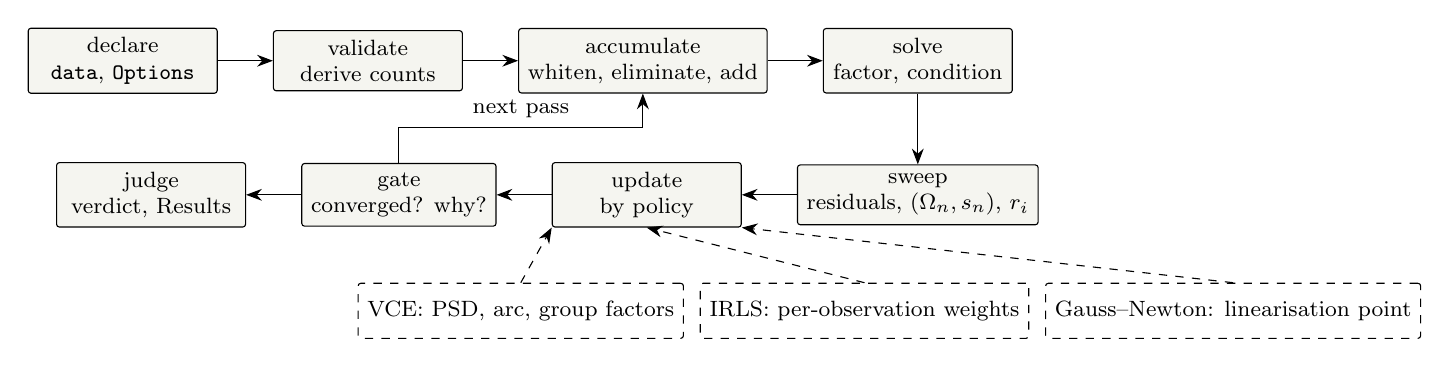
\begin{tikzpicture}[node distance=9mm and 7mm, every node/.style={font=\footnotesize},
  box/.style={draw,rounded corners=1pt,minimum height=7mm,minimum width=24mm,align=center,fill=boxbg},
  pol/.style={draw,dashed,rounded corners=1pt,minimum height=7mm,align=center},
  >={Stealth[length=2mm]}]
\node[box] (decl) {declare\\\code{data}, \code{Options}};
\node[box,right=of decl] (val) {validate\\derive counts};
\node[box,right=of val] (acc) {accumulate\\whiten, eliminate, add};
\node[box,right=of acc] (sol) {solve\\factor, condition};
\node[box,below=of sol] (swp) {sweep\\residuals, $(\Omega_n,s_n)$, $r_i$};
\node[box,left=of swp] (upd) {update\\by policy};
\node[box,left=of upd] (gate) {gate\\converged? why?};
\node[box,left=of gate] (jud) {judge\\verdict, Results};
\draw[->] (decl)--(val); \draw[->] (val)--(acc); \draw[->] (acc)--(sol); \draw[->] (sol)--(swp);
\draw[->] (swp)--(upd); \draw[->] (upd)--(gate); \draw[->] (gate)--(jud);
\draw[->] (gate.north) -- ++(0,4.5mm) -| node[pos=0.25,above]{next pass} (acc.south);
\node[pol,below=7mm of upd,xshift=-16mm] (p1) {VCE: PSD, arc, group factors};
\node[pol,right=2mm of p1] (p2) {IRLS: per-observation weights};
\node[pol,right=2mm of p2] (p3) {Gauss--Newton: linearisation point};
\draw[->,dashed] (p1.north) -- (upd.south west); \draw[->,dashed] (p2.north) -- (upd.south); \draw[->,dashed] (p3.north) -- (upd.south east);
\end{tikzpicture}
\end{center}

\code{Model="gls"} is the loop with an empty policy (one pass, judge). The policies compose: a nonlinear problem with VCE runs both updates per pass (the ITSG scheme does exactly this: re-linearised orbits and re-estimated covariance functions in the same iteration).

\section{The pass record}

Each pass leaves a row in \code{R.history}: the pass number, wall time per step, the update norms per component, the whiteness statistics per stream, the arcs skipped with their reason counts, the condition evidence, and the gate decision with its reason. The row is what \code{R.convergence()} tabulates and what a warning names when the budget is exhausted. It is written \emph{before} the next pass starts, so an interrupted run is diagnosable.

\section{Collectors in the sweep}

The residual sweep carries a list of collectors, each with \code{init}, \code{accumulate(arc, context)} and \code{fold(a, b)}; the fold is associative and applied in day order. The v5 collectors: whitened residual norms per group; per-lag $(\Omega_n, s_n)$ per stream (exact or probe); per-observation $r_i$, $w_i$ and the worst-$K$ heap (exact route); the whiteness autocorrelations per stream; the group contributions. A collector that is not needed by the policy or the requested diagnostics is not attached --- the sweep's cost is the sum of its collectors, and the report lists which ran.

\section{The accumulator}

One class, \code{engine.Accumulator} (the v5 name for today's \code{BlockAccumulator}; the flat batch accumulator is retired), with: a backend (NEQ or QR), a common block of size $u$, one store per system holding the current scope's local block and its Schur-complement machinery, \code{addArc}, \code{closeScope} (eliminate the local block of a day or a system when its last arc has been added), \code{solve}, \code{backSubstitute}, \code{condition}. A ``batch'' problem is a system with one day, one arc per batch and $n_l = 0$; a nonlinear problem re-linearises by calling the builder with the current $\vc x$. The class is the only place that knows the backend.

\section{Layers and the call rule}

\begin{tabular}{@{}P{16mm}P{104mm}P{34mm}@{}}
\toprule
tier & contents & calls\\
\midrule
USER & \code{fit}, \code{Options}, \code{Results}, \code{report} & ENGINE\\
ENGINE & loader, accumulator, iteration, sweep, VCE, diagnostics, provenance & KERNEL, UTIL\\
KERNEL & transforms, filters, recursions, statistics --- pure functions on arrays & UTIL\\
UTIL & logging, verbosity, struct helpers & ---\\
\bottomrule
\end{tabular}

Calls go downward only; a KERNEL function takes arrays and returns arrays, prints nothing and reads no option object. The layering is declared in one table (\code{tiers.csv}) and checked by the audit (check 18). A function that a USER-tier verdict tells the user to run is itself USER-tier reachable through \code{Results} (Part IV, H-05).

\chapter{Error handling}
\label{ch:errors}

Error handling in an estimation toolbox is not exception plumbing; it is the set of rules that decide \emph{which number the user is allowed to see}. The rules below are binding for v5 and are checked mechanically where a check is possible (Part V, WP-M1).

\section{Three outcomes and no fourth}

Every operation ends in exactly one of: \textbf{refuse} (an error with a documented identifier, nothing returned), \textbf{report} (a result plus a warning naming what was assumed or skipped), or \textbf{proceed} silently (nothing was assumed). A fourth outcome --- proceed silently on an assumption --- is the defect class this chapter exists to remove. Corollaries:
\begin{itemize}
\item No function returns a numeric status code; status is either an exception or a named field of the result that the report prints.
\item No empty \code{catch}. A \code{catch} either re-throws with the original as \emph{cause} (\code{MException.addCause}), or converts a \emph{named} expected failure into a recorded skip (\S\ref{sec:skips}). A bare \code{catch} that converts \emph{any} error into a default also converts an undefined variable into a wrong answer.
\item A \code{NaN} where a number belonged is the worst outcome, \emph{except} when NaN is the honest value of a quantity that cancelled in double precision --- then it is the only outcome, it carries one identifier, and the report explains it (\S\ref{sec:cancellation}).
\end{itemize}

\section{Identifiers}

\code{lsqvce:<unit>:<reason>}, unit = the function or class that raises, reason in lowerCamelCase. The documented identifier equals the raised one, enforced by a static check that parses every \code{error(}/\code{warning(} site and every help ERRORS block. The catalogue (Appendix~\ref{app:ids}) is the \emph{authority}: a new identifier is added to the catalogue in the same commit, and the audit refuses an identifier raised but not catalogued. Refusals raised on the user's behalf by the engine keep the engine's unit (\code{lsqvce:makeLoader:dayShape}), because that is where the evidence is; refusals of the declaration are raised by \code{fit} before any read.

\section{Refusal catalogue: what is refused, and with what evidence}

\begin{longtable}{@{}P{30mm}P{54mm}P{70mm}@{}}
\toprule
class & refused when & the message must carry\\
\midrule
declaration & an unknown field, a missing required field, a scope token misuse, a duplicate id, a non-integer day, an arc id out of range & the field name, the system index/id, the rule violated (one identifier per rule)\\
builder output & missing \code{A}/\code{B}/\code{l}/\code{t}; row counts disagree; column counts disagree with the derived nc/nl; \code{arcId} does not partition & day, observation type, system, expected vs found sizes\\
builder threw & any exception inside the user's function & day, observation type, system; the user's exception as cause, unmodified\\
covariance law & non-PD Toeplitz; sigma $\le 0$; AR polynomial with roots on/inside the unit circle; law length shorter than the longest arc; $\Delta t$ missing for a time-domain law & the stream, the offending lag/root/length, and the remedy (PSD form, taper, longer law)\\
rank & trailing pivot ratio below $\epsilon$; null-space dimension $d>0$ without a datum & $d$, the parameters with the smallest pivots, the backend, and the QR/regularisation remedy\\
estimability & a component whose redundancy is below the freeze threshold on the \emph{first} pass with no prior value & the component key and its $r_g$\\
cancellation & $\Omega$ below the cancellation floor on the normal-form path with no residual sweep to supersede it & $\hat\sigma_0 = $ NaN as a \emph{result}, one identifier, the floor and both operands in the diagnostics\\
options & a value outside its enum/range; a combination that is contradictory (\code{DistributeDays} without a parallel policy; arc factors on a \code{diag} law) & the property, the value, the allowed set; for combinations both properties\\
\bottomrule
\end{longtable}

\section{Skips are results}
\label{sec:skips}

An arc that cannot be whitened (non-PD law after an update), a day the resolver declares but the builder does not carry, a component that is frozen this pass --- these are expected in production and are \emph{skips}, not errors. Each skip has a reason code from a closed list, is counted per pass and per stream, and the first instance's message is kept. The pass record carries the counts; the report prints them; and a \emph{threshold} turns a skip rate into a refusal (more than a declared fraction of arcs skipped in a stream $\Rightarrow$ the stream's law is refused, the run stops with the reason). A skip that nobody counts is the silent-degradation outcome in disguise.

\section{Warnings}

One identifier per situation; it fires \emph{once per run}, not once per arc (the count is in the skip record); the inventory of identifiers fired is stored in \code{R.meta.warnings} and printed by the report. A test that provokes a documented warning disables that identifier for its duration with a cleanup-based restore; a clean run's inventory contains at most the one deliberate probe identifier (VALIDATION\_GUIDE Part 5). Library code never prints: every message goes through \code{util.log} under one verbosity control.

\section{Convergence is a result}

Reaching the pass budget, alternating components, or a stream that never whitens are outcomes of the estimation, not failures of the code. They set \code{R.converged = false}, \code{R.stopReason} from a closed enum (\code{"tolerance"}, \code{"whiteness"}, \code{"maxPasses"}, \code{"alternating"}, \code{"skipThreshold"}), and one warning. The estimates of the last pass are returned with their covariance; the report's level-1 line says which criterion stopped the loop. Refusing to return a non-converged estimate would hide exactly the evidence the user needs.

\section{User functions}

The builder, the arc resolver, the epoch-covariance hook and any plot hook are user code. They are called through one wrapper that (i) checks the declared \code{nargin}/\code{nargout} \emph{once} with \code{nargin(fh)}/\code{nargout(fh)} rather than by catching \code{MATLAB:TooManyOutputs} on every call (Part IV, H-08), (ii) wraps any exception with the call context and the original as cause, and (iii) validates the returned struct against the contract before it reaches the engine. A plot hook that throws is reported and disabled for the rest of the run; a builder that throws refuses the run.

\section{Parallel execution}

A worker error carries the day and system it was processing and is re-thrown on the client with that context; a pool that cannot be opened is a \emph{report} (warning naming the reason, serial fallback), never a silent \code{info.fallback} string; the fold order is fixed; a serial re-run of a failing day is the documented first diagnostic step. Logging from workers is collected through one queue and emitted in day order.

\section{What the tests must prove}

Every identifier in the catalogue fires in a contract test, and only that one fires (a rejected call must not trip a different check first). Every skip reason is provoked once and shown to reach the report. The bare-\code{catch} count in the tree is an audit metric with a target of zero. The warning-once property is asserted with a counter over a large $N$. These are the \code{contract} and \code{robustness} categories of Part V applied to the error surface.

\part{Review R5 of \lsq{} v4.0}
\begin{principle}[Dated record]
This Part and the two that follow describe the tree of 1 September 2026 (v4.0) and the v5 plan. For the implemented state see the Manual and \code{RELEASE\_NOTES.md} (R6 WP-106).
\end{principle}

\chapter{Method, scope, and what is right}
\label{ch:review}

\section{Method}

The panel read the tree at \code{main} head \code{d7ad051} (2026-09-01: v4.0, 83 public names in \code{+lsqvce}: USER 4 / ENGINE 58 / KERNEL 21; 26\,054 lines of package code; 23 suites, 634 declared test points, CI green; postflight green 622/622 on R2026a) with the Ellmer (2018) and Kvas (2019) theses and the \code{referenceSystem} guides (\code{CODING\_GUIDE}, \code{VALIDATION\_GUIDE}, \code{DOCUMENTATION\_GUIDE}) open beside it, and the R2--R4 reviews of \code{dev/HANDOVER.md} as the record of what had already been found. Instruments: a code-only call-graph (comments and string literals stripped) rooted at the four USER names; the audit's own category matrix; a census of every \code{catch} block; a reading of \code{fit}, \code{Options}, \code{Results}, \code{adjustVCE}, \code{adjustVCEjoint}, \code{BlockAccumulator}, \code{makeLoader} and \code{DATA\_CONTRACT.md} in full. Where a claim rests on running MATLAB (timing, numerical parity) it is marked PREDICTED; everything else is repo-verified with a file and line.

\section{What R5 confirms as right}

These stay; none of Part V touches them:
\begin{enumerate}
\item \textbf{The Ellmer path is complete and correct in structure.} \code{fit(Model="ellmer")} $\to$ \code{adjustVCEjoint} $\to$ \code{psdVCE} (eq. 6.5.19--21), \code{arcVarianceFactors} (6.5.27--30, robust mean, clamp), \code{kernel.redundancyLags} (6.5.22--23 with the local projector of WP-33), \code{sharedProbe}/\code{probeMatrix} (6.5.48, one $\mat U^{-1}\bar{\mat Z}$ per pass), \code{kernel.dctI} (6.5.25--26). This is the core the redesign builds on; it becomes the \emph{only} stochastic-model estimator.
\item vTv honesty (NaN on cancellation, one identifier, both backends); NEQ default with QR fallback and visible condition evidence; the WP-36 probe contract with seeds in the provenance.
\item The v4 data contract's principle --- state nothing the data already states; scope, don't number --- and the block-arrow accumulator with per-scope elimination and deterministic day-order folds (WP-62).
\item Run provenance (\code{R.meta}), the six-category test taxonomy with the countability gate, the tolerance-provenance rule (0 unannotated tolerances), the physically structured oracle (WP-48) and the metamorphic suite (WP-29).
\item The level-based development loop, the audit as a merge gate, and the honesty invariants pinned in HANDOVER §11.2.
\end{enumerate}

\chapter{Findings H-01 \ldots H-14}
\label{ch:findings}

Each finding: evidence, verdict of the three experts, disposition (the work package of Part V that addresses it).

\section*{Design flaws and superfluous paths}

\finding{H-01 Twenty-four package files are not reached by any code path from the USER surface.} Code-only call graph from \{\code{fit}, \code{Options}, \code{Results}, \code{report}\}: unreached are \code{engine.Combine} (1070 lines), \code{BatchIndex} (470), \code{varComp} (503), \code{vceHutchinson} (379), \code{iterateNoiseModel} (315), \code{selectArOrder} (216), \code{PrefetchLoader} (221), \code{synthLoader} (257), \code{poolGroups}, \code{resolveSatSpecs}, \code{normalizeSatList}, \code{checkPSD}, \code{ftest}, \code{ellipse}, \code{datum}, \code{CommonPrior}, \code{snoop}, \code{systematic}, \code{kernel.crossCorr}, \code{toeplitzCofactor}, \code{covComponent}, \code{whitenessCorr}, \code{whittle}, \code{util.hasBackgroundPool}. None of them is on the Ellmer path (previous section). They fall into three classes: (i) \emph{duplicates} of a live implementation --- \code{Combine}/\code{BatchIndex} (v1 multi-dataset combination, superseded by \code{BlockAccumulator}; only caller \code{test\_lsqvce\_combine}, 27 points), \code{varComp}/\code{vceHutchinson} (Helmert VCE on the flat batch path that \code{fit} refuses for \code{Model~="gls"}, \code{fit.m:577}), \code{iterateNoiseModel}/\code{selectArOrder} (an older AR-order loop; \code{adjustVCE} uses \code{selectArAcv}); (ii) \emph{instruments} that should run as part of the verdict or the tests but are only reachable by the user typing their name --- \code{snoop}, \code{systematic}, \code{datum}, \code{checkPSD}, \code{ftest}, \code{ellipse}, \code{CommonPrior}, \code{covComponent}/\code{toeplitzCofactor} (the $\mat V_n$ of eq. 6.5.16); (iii) \emph{experiments} with no measured benefit on record --- \code{PrefetchLoader}, \code{poolGroups}, \code{synthLoader} (a template that G-06 showed drifts from the engine). \textit{Verdict:} class (i) is deleted (no aliases), class (ii) moves into the sweep/verdict or into \code{dev/tests}, class (iii) is deleted unless a measurement in WP-M0 shows a benefit. About 5\,000 lines and 5 test suites leave the tree. \textit{Disposition:} WP-M0, WP-M2.

\finding{H-02 Two accumulators, two diagnostics entries, two Helmert implementations.} \code{engine.Accumulator} (713, flat batches, diagonal weights) and \code{engine.BlockAccumulator} (1284, block-arrow, streaming) implement the same normal-equation/QR accumulation twice; \code{engine.diagnose} (1016) computes per-observation diagnostics for the flat path while \code{diagnoseAccum} (235) bridges the streaming path into it; \code{fit} kinds B/C dispatch to \code{adjust}/\code{robust}/\code{solveNonlinear} on the flat accumulator, kind A to \code{adjustBlock}/\code{adjustVCE}/\code{adjustVCEjoint} on the block one (\code{fit.m:273--291, 583--626}). A batch problem is a streaming problem with one day, one arc per batch and $n_l=0$ (Chapter~\ref{ch:impl}); the flat path adds nothing but a second code base to keep in parity. \textit{Verdict:} one accumulator; kinds B/C become adapters that generate a \code{buildDay} from \code{A/l/p} or \code{batchFcn}. \textit{Disposition:} WP-M2.

\finding{H-03 Three stochastic-model estimators, one of them an unjustified approximation.} \code{adjustVCE} (2541 lines, the largest file; \code{run} + \code{applyShape} + \code{applyScale} + \code{applyJoint}) carries mode \code{separate} (Helmert group scale over \code{GroupBy} groups \emph{plus} an AR law per stream fitted to the \emph{raw residual autocovariance}, \code{biasedAcv}/\code{biasedAcvAxes}, \code{adjustVCE.m:1809, 2237}) and mode \code{joint} (pooled PSD by per-lag VCE); \code{adjustVCEjoint} carries the Ellmer scheme. The residual ACV is a biased estimate of the noise ACV --- $\E[\bar{\vc v}\bar{\vc v}\T] = \sigma^2\mat R \ne \sigma^2\mat I$ --- with a bias of order $\tr(\bar{\mat H})/m$ per arc, which is small only when $m_a \gg u_{\text{local}}$ and the common-block leverage is small. On GRACE arcs ($m\approx 2000$, $n_l\approx 6$--12) the bias is percent-level at low lags and grows where the local model absorbs low frequencies --- exactly the frequencies that decide the KBR weight. The per-lag redundancy $s_n$ that removes this bias is computed by the same tree (\code{redundancyLags}) for the other two modes. \textit{Verdict (Expert A):} the deviation is not justified in general and is unnecessary, since the exact machinery exists; the AR route is kept as a \emph{whitener choice} (a reduction of the estimated PSD, \S\ref{sec:whitening}), not as an estimator. \textit{Verdict (Expert B):} one estimator with two switches --- pooling scope and arc factors --- reproduces all three modes. \textit{Disposition:} WP-M3 (with a parity test: the new single estimator equals today's \code{ellmer} output on the WP-51 fixture to $10^{-10}$, and equals \code{pooled} with arc factors off).

\finding{H-04 Sweeps are duplicated instead of collected.} The residual pass (\code{engine.residuals}), the redundancy pass (\code{engine.redundancy}, with its own \code{mapreduce}), the per-lag pass (\code{adjustVCE.sweepStreamLags}, \code{adjustVCE.m:1571}), the whiteness ACV, the contribution probes (\code{streamContribution}) and the outlier screening (\code{outliers}/\code{snoop}) each re-read and re-whiten the arcs. The v2 design (HANDOVER §3.5, WP-10 ``sweep --- the ONE second data pass with collectors'') was reconciled as done in 2026-08-16 but was never realised in this form. \textit{Verdict:} one sweep with attachable collectors (Chapter~\ref{ch:impl}); PREDICTED saving per VCE pass: 2--4 re-reads of every arc. \textit{Disposition:} WP-M4.

\finding{H-05 The verdict tells the user to run engine functions.} \code{report.m:286} prints ``Run \code{lsqvce.engine.systematic()} and fix the functional model''; \code{report.m:425} ``re-snoop --- \code{lsqvce.engine.snoop()} does this for you''; \code{robust.m:292}, \code{snoop.m:257/336/351} likewise. The USER tier hands the user an ENGINE name. \textit{Verdict (Expert C):} the systematic-error test and the snooping are collectors of the sweep and methods of \code{Results} (\code{R.systematic()}, \code{R.snoop()}); the verdict names the method. \textit{Disposition:} WP-M4, WP-M5.

\finding{H-06 The PSD grid is sized by probing data inside a \code{try}.} \code{adjustVCE.covGridSize} (\code{adjustVCE.m:1395--1466}) calls the loader for the first day and arc, catches \emph{any} error and sets \code{mMax = 0}, then defaults the grid to 128 frequencies. The longest arc is a property of the declared schedule (the resolver) and of the read days (enforced by the accumulator, which sees every arc). \textit{Verdict:} R3 of the coding guide --- measured, never probed and defaulted. \textit{Disposition:} WP-M3 (grid = the longest arc seen in pass 1, recorded in the pass record; a user override is a declared choice).

\section*{Error handling}

\finding{H-07 Five empty \code{catch} blocks and thirteen bare \code{catch} defaults.} Census of the 36 \code{catch} sites: empty --- \code{adjustVCE.m:1456} (keep a guessed grid), \code{adjustVCE.m:2050} (\code{ctx.sd = []}), \code{BlockAccumulator.m:586} (no local covariance in the log), \code{util/log.m:196}, \code{util/showExport.m:63}; bare \code{catch} $\to$ default --- \code{BlockAccumulator.m:577} (\code{continue}: ``system not recoverable''), \code{adjustVCE.m:1432, 1513, 1566, 2116, 2329, 2332}, \code{PrefetchLoader.m:184, 198}, \code{gcvLambda.m:62}, \code{log.m:123, 218, 225, 306}, \code{hasBackgroundPool.m:47}, \code{showExport.m:93}, \code{mapreduce.m:205} (pool failure becomes an \code{info.fallback} string). Each converts an undefined variable, a typo or a shape error into a silently different run. \textit{Verdict:} Chapter~\ref{ch:errors} \S1; every site is rewritten as refuse-or-record; the audit counts bare \code{catch} and targets zero. \textit{Disposition:} WP-M1.

\finding{H-08 Output-arity probing by exception, five times.} \code{adjust.m:156}, \code{robust.m:306}, \code{solveNonlinear.m:317}, \code{Combine.m:1013}, \code{adjustVCE.m:1977} each call the user's function and catch \code{MATLAB:TooManyOutputs}/\code{maxlhs}/\code{unassignedOutputs} to learn how many outputs it returns --- on \emph{every} call, and a user function that itself raises one of these identifiers is misread. \textit{Verdict:} one wrapper, \code{nargout(fh)} once at declaration time. \textit{Disposition:} WP-M1.

\finding{H-09 369 error identifiers in 40+ unit namespaces, 90 of them in files that H-01 deletes.} \code{lsqvce:combine:} (24), \code{lsqvce:batchIndex:} (17), \code{lsqvce:varComp:} (9), \code{lsqvce:vceHutchinson:} (7), \code{lsqvce:iterateNoiseModel:} (6), \code{lsqvce:ftest:} (6), \code{lsqvce:checkPSD:} (4), \code{lsqvce:toeplitzCofactor:} (3), \ldots; the same rule is raised under different units (\code{lsqvce:accum:} 28 vs \code{lsqvce:acc:} 22 for the two accumulators). There is no catalogue and no documented-equals-raised check (the audit's check 15 verifies ids appear in help, not that the catalogue is closed). \textit{Disposition:} WP-M1 (catalogue, Appendix~\ref{app:ids}; target $\approx 130$ identifiers).

\finding{H-10 Skips are counted in some places and not others.} \code{adjustVCEjoint} counts \code{skip.cfcnErr}/\code{wfcnErr} with the first message (good); \code{adjustVCE.applyShape} logs an epoch-covariance failure only at detail verbosity and proceeds on the scalar fallback (\code{adjustVCE.m:1793}), which is precisely the biased path the L10 rationale warns about; \code{BlockAccumulator.logLocalSummary} drops a system silently. No skip rate is ever turned into a refusal. \textit{Disposition:} WP-M1, WP-M4 (closed skip enum, threshold).

\section*{Interface}

\finding{H-11 One options object, 57 flat properties, three problems mixed.} \code{Options.m} declares 57 typed properties in ten help groups; the batch-only (\code{DatumB}, \code{Sigma0}, \code{Sparse}, robust, nonlinear), streaming-only (\code{GroupBy}, \code{DistributeDays}, Shape/Scale/Outer) and joint-only (\code{NumLags}, \code{StepSchedule}, \code{AvgTail}) knobs sit side by side, and \code{Model} conflates ``iterate or not'' with ``which estimator'' (\code{gls}/\code{vce}/\code{pooled}/\code{ellmer}). A new user reads 57 rows to find the four that matter. \textit{Verdict (Expert C):} the stock-MATLAB shape is a small top-level object with typed \emph{groups} (\code{fitlm}'s \code{RobustOpts}, \code{optimoptions}' solver-specific sets): $\approx 12$ top-level properties, plus \code{Noise}, \code{Robust}, \code{Diagnostics}, \code{Parallel} groups; \code{Model} splits into what is estimated (\code{Estimate}) and how the loop stops. \textit{Disposition:} WP-M5, decision R5-D2.

\finding{H-12 The stochastic-model choice lives in two places.} What is estimated for a stream is decided by \code{Options.Model} (global), while the a-priori law lives in \code{data.systems(k).covariance.(obsType)} (per stream). A stream with a trusted \code{diag} law and a stream with an unknown red spectrum cannot be treated differently in one run. \textit{Verdict:} the covariance spec gains one field, \code{estimate = "none" | "scale" | "law"} (+ \code{arcFactors}, \code{pool}), so the declaration says per stream what is free; \code{Options} keeps only run-level policy. \textit{Disposition:} WP-M5, decision R5-D3 (a v5 contract change --- additive fields, one breaking rename at most).

\finding{H-13 \code{fit} accepts only an \code{Options} object; \code{Results} has no plot; README shows retired names.} \code{fit(data, opts)} requires constructing \code{lsqvce.Options} first; stock functions take Name-Value directly. \code{Results} has \code{report}/\code{coefficients}/\code{convergence}/\code{summary} but no \code{plot} --- the estimated PSD per stream and the pass trajectory are the two pictures every user needs, and both are available in \code{R.noise}/\code{R.history} without a design matrix (the WP-57 omission argued about \code{predict}, which stays omitted). \code{README.md:60} shows \code{systemId} and \code{localsPerArc}, both retired in L10/L11. \textit{Disposition:} WP-M5 (\code{fit(data, Name=Value)} via a positional \code{opts} \emph{and} \code{nv.?lsqvce.Options}; \code{plot(R, "psd"|"convergence"|"residuals")}), WP-M6 (docs).

\section*{Tests}

\finding{H-14 Category coverage: 3 of 83 units complete, 47 missing three or more categories; metamorphic is a tag; speed budgets are absolute.} Audit check 16 (informational, 245 gaps): \code{report} has contract tests only; \code{Results} lacks speed and vectorisation; the USER-tier \code{fit} lacks vectorisation. The WP-29 metamorphic suite exists but is not a counted category. \code{test\_speed} carries absolute budgets and runs locally only. \textit{Verdict:} adopt the seven-category scheme and ratio budgets of \code{VALIDATION\_GUIDE} (Part V, Chapter~\ref{ch:tests}); with H-01/H-02 the unit count drops to $\approx 45$, so completeness becomes affordable. \textit{Disposition:} WP-M0 (harness first), WP-M7.

\chapter{Limitations of the method (to document, not to fix)}
\label{ch:limits}

\begin{enumerate}
\item \textbf{Stationarity per arc and month.} Non-stationary noise (eclipse transitions, thruster events) is absorbed by arc factors at arc resolution only.
\item \textbf{Signal--noise ambiguity.} Unmodelled signal is down-weighted as noise (\S\ref{sec:vcelimits}); no estimator can tell them apart without a functional model of the signal.
\item \textbf{Monte-Carlo redundancy.} $\pm\sqrt{2/Z}$ relative on each trace; no per-observation reliability on the probe route.
\item \textbf{Local absorption.} Per-arc empirical parameters remove low-frequency noise power from the estimated law; the law describes the residual process, not the instrument.
\item \textbf{Identifiability of nested factors.} Arc and day factors on the same stream are not separable; the contract forbids it, and the theory has nothing better.
\item \textbf{Simplified Helmert.} The Förstner iteration ignores the off-diagonal Helmert terms; it converges to the same fixed point but does not deliver the full covariance of the components --- only the diagonal Fisher bound is reported.
\item \textbf{Scale of $u$.} Dense $u\times u$ blocks bound the common parameter count to $\sim 2\cdot10^4$ on a workstation; beyond that, out-of-core or sparse block strategies are a different toolbox.
\item \textbf{Gaps.} Cut, not modelled; the Toeplitz structure is per contiguous arc.
\end{enumerate}

\chapter{The panel's discussion}
\label{ch:discussion}

\begin{panel}[On collapsing the three noise estimators (H-03)]
\textbf{A:} The Ellmer per-lag estimator is the correct one and we already have it; the residual-ACV shortcut was a v1 convenience that survived because it converges to something plausible. Keep the AR reduction as a whitener, not as an estimator.\\
\textbf{B:} Agreed, with one condition: the ``separate'' mode is what people run when they have one satellite and 30 days --- it must stay \emph{fast}. The per-lag route with probes costs one $u\times Z$ solve per pass and $O(mZ)$ per arc; at $u=4000$ that is cheaper than the exact leverage the separate mode computes today for its Helmert step. So the unification is a speed-up, not a cost. PREDICTED; WP-M3 measures it.\\
\textbf{C:} And it deletes \code{applyShape}/\code{applyScale}/\code{applyJoint} and half of \code{adjustVCE}. The parity test is the risk: today's \code{vce} mode has no reference other than itself. We pin the new estimator against \code{ellmer} (which has the Python mirror of \code{v10review.py}) and accept that \code{vce}-mode outputs \emph{change} --- that is a breaking release and it is the right one.
\end{panel}

\begin{panel}[On the batch kinds (H-02)]
\textbf{C:} Kinds B and C exist so that a levelling network or a GNSS batch can use the same verdict. They are a system with one day. Folding them costs one adapter of 60 lines and removes 2\,500.\\
\textbf{A:} The robust IRLS then becomes available on the streaming kind, which it is not today (\code{lsqvce:fit:notYet}). That is a feature, not a side effect.\\
\textbf{B:} One caution: the block accumulator's per-arc overhead (arc validation, local-block bookkeeping) must not be paid per row of a 10-row batch. The adapter groups batches into arcs of the user's size; the speed test pins the dispatch ratio.
\end{panel}

\begin{panel}[On the options object (H-11, H-12)]
\textbf{C:} 57 flat properties is what happens when every driver's Name-Value list is unioned. The user-facing set is: what to estimate, how many passes, when to stop, how to parallelise, how loud. Everything about a stream belongs with the stream.\\
\textbf{B:} Per-stream \code{estimate} also fixes a real workflow: ACC-derived streams have a law we trust from the instrument team; KBR does not. Today one \code{Model} rules both.\\
\textbf{A:} And a prior (regularisation) is a stream with \code{estimate="scale"}. Then there is nothing special about \code{Reg} either; it is a group.
\end{panel}

\begin{panel}[On how much to simplify]
\textbf{C:} Every deletion is a breaking change and the tree has had four breaking releases in a month. Is a fifth right?\\
\textbf{B:} The four were about the \emph{declaration}, which is now good and stays (R5-D1: the v4 contract is kept, extended additively). v5 is about the \emph{engine} and the options. Users of \code{fit}+\code{data} see a smaller \code{Options}, a per-stream \code{estimate} field, and better numbers; they do not rewrite a builder.\\
\textbf{A:} The one thing that must not be simplified away is the evidence: probe counts, redundancies, skips, condition numbers. Fewer knobs, not fewer numbers.
\end{panel}

\part{The redesign: \lsq{} v5}

\chapter{Design principles and the logic}
\label{ch:design}

\begin{principle}[Six principles, in order of precedence]
\begin{enumerate}
\item \textbf{One estimator, one loop, one accumulator, one sweep.} Every variance component is $\Omega/r$; every iteration is accumulate--solve--sweep--update--gate; every problem kind enters through the same accumulator; every second read is the sweep with collectors.
\item \textbf{Declaration says what is free; options say how to run.} What is estimated for a stream is a property of the stream (\code{estimate}); the pass budget, tolerances, probes, parallel axis and verbosity are properties of the run.
\item \textbf{Refuse, report, or proceed.} Chapter~\ref{ch:errors}, mechanically checked.
\item \textbf{Measured, never probed.} Every count and grid comes from the declaration or from what was read and enforced; no defaults behind a \code{try}.
\item \textbf{Fewer knobs, not fewer numbers.} Evidence (redundancy, probes, skips, condition, warnings) is always in the result.
\item \textbf{Stock-MATLAB ergonomics.} \code{R = lsqvce.fit(data, Name=Value)}; \code{plot(R)}; \code{disp(R)}; typed option groups; identifiers a user can \code{try/catch}.
\end{enumerate}
\end{principle}

\section{The logic, top down}

\begin{lstlisting}
R = lsqvce.fit(data, opts)
  D    = engine.declaration(data)   % validate, derive nc/nl/arcs, one Loader per system
  P    = engine.policy(D, opts)     % which components are free, which updates run
  noise= engine.noise.init(D)       % per-stream law: PSD grid, whitener, arc factors = 1
  acc  = engine.Accumulator(D.nc, opts.Backend)
  for pass = 1:opts.MaxPasses
      acc.reset();
      engine.accumulate(acc, D, noise, opts.Parallel)   % parallel over days, fold in day order
      sol  = acc.solve();                                % factor, condition, NaN-honest sigma0
      S    = engine.sweep(acc, D, noise, sol, P.collectors, opts.Parallel)
                                                         % residuals, (Omega_n, s_n), r_i, whiteness, worst-K
      [noise, x0, upd] = engine.update(P, noise, S, sol) % VCE / IRLS / Gauss-Newton, in that order
      hist(pass) = engine.passRecord(pass, sol, S, upd) % skips, norms, whiteness, timing, gate
      if engine.gate(hist, opts), break, end
  end
  R = lsqvce.Results(sol, S, hist, noise, D, engine.runMeta(opts))   % verdict on demand: R.report
\end{lstlisting}

\code{Model="gls"} is \code{MaxPasses = 1} with an empty policy; every other model is a policy. The batch kinds are \code{engine.declaration} recognising \code{A/l/p} or \code{batchFcn} and synthesising one system with a generated \code{buildDay}.

\chapter{The user interface}
\label{ch:ui}

\section{Three lines, all kinds}

\begin{lstlisting}
R = lsqvce.fit(data);                                   % GLS under the declared laws
R = lsqvce.fit(data, Estimate="noise", MaxPasses=8);    % VCE: laws, arc factors, group scales as declared
R = lsqvce.fit(data, Estimate="noise", Robust="huber");  % plus IRLS on the same loop
R = lsqvce.fit(struct(A=A, l=l, p=p), Robust="igg3");   % an in-memory problem, same verdict
R.report;  T = R.coefficients;  plot(R, "psd");  plot(R, "convergence")
\end{lstlisting}

\section{\code{lsqvce.fit}}

\begin{lstlisting}
function R = fit(data, opts, nv)
arguments
    data (1,1) struct
    opts (1,1) lsqvce.Options = lsqvce.Options()
    nv.?lsqvce.Options                        % Name=Value overrides, stock-MATLAB style
end
\end{lstlisting}
The positional \code{opts} and the Name-Value overrides are \emph{one} mechanism (the overrides are applied to \code{opts} and validated by the class); the recorded \code{R.meta.options} is the resolved object. Errors of the declaration carry \code{lsqvce:fit:<rule>}; nothing is read before validation completes.

\section{\code{lsqvce.Options} --- twelve properties and four groups}

\begin{longtable}{@{}P{28mm}P{34mm}P{90mm}@{}}
\toprule
property & type / default & meaning\\
\midrule
\code{Estimate} & \code{"none"} $|$ \code{"noise"} & \code{"none"}: one GLS pass under the declared laws. \code{"noise"}: run the VCE policy on every stream whose spec declares something free (\code{estimate ~= "none"}). Replaces \code{Model}; the pooled/ellmer distinction moves to the stream spec.\\
\code{Robust} & \code{"none"} $|$ \code{"huber"} $|$ \code{"igg3"} $|$ \code{"bisquare"} & IRLS policy on the same loop; details in \code{Robust} group\\
\code{MaxPasses} & 8 & outer pass budget (1 for \code{Estimate="none"})\\
\code{Tolerance} & 5e-3 & stop when every free component moved less than this (relative)\\
\code{Whiteness} & 0.01 & Ljung--Box level; a stream is ``white'' above it; stop when all are\\
\code{Backend} & \code{"normal"} $|$ \code{"qr"} & \S\ref{sec:twosolvers}\\
\code{Probes} & 100 & Hutchinson probes for the per-lag redundancies; \code{0} = exact route\\
\code{Seed} & [] & RNG seed for the probes; recorded\\
\code{Parallel} & group & \code{Mode "auto"|"serial"|"pool"}, \code{Axis "days"|"arcs"}, \code{Threshold 8}\\
\code{Noise} & group & \code{Grid} (\code{"auto"} = longest arc), \code{Whitener "toeplitz"|"ar"}, \code{MaxOrder 60}, \code{Floor 1e-3}, \code{Smooth 0}, \code{MeanType "robust"|"plain"}, \code{FreezeRedundancy 1}, \code{SkipThreshold 0.2}\\
\code{Robust} & group & \code{Tuning [] (= influence default)}, \code{MaxIter 30}, \code{Tol 1e-8}\\
\code{Diagnostics} & group & \code{Alpha 1e-3}, \code{Bonferroni true}, \code{Beta 0.2}, \code{RWeak 0.1}, \code{Test "auto"|"pope"|"baarda"}, \code{Store "flagged"|"all"|"none"}, \code{NWorst 1000}, \code{Systematic true}\\
\code{Verbose} & 1 & 0..3\\
\code{LogFile} & "" & path; "" = none\\
\bottomrule
\end{longtable}
Regularisation is not an option: a prior is a stream (\S\ref{sec:contractdelta}). Nonlinear is not an option: \code{data.x0} declares it. \code{DistributeDays}, \code{ParallelThreshold}, \code{GroupBy}, \code{VceMode}, \code{NumLags}, \code{Norm}, \code{StepSchedule}, \code{AvgTail}, \code{C0}, \code{PsdMode}, \code{ComponentsPerEpoch}, \code{DatumB}, \code{Sigma0}, \code{Sparse}, \code{Reg*}, \code{ShowSeconds}, \code{ExportDir}, \code{LogFid}, \code{LogFlag} and the \code{Vce*}/\code{Joint*}/\code{Nonlinear*}/\code{Outer*} names leave; Appendix~\ref{app:mapping} maps each.

\section{The data contract, v5 delta}
\label{sec:contractdelta}

The v4 struct stays (R5-D1). Additive changes only:
\begin{itemize}
\item \code{covariance.(obsType).estimate} $\in$ \{\code{"none"}, \code{"scale"}, \code{"law"}\}, default \code{"none"}. \code{"scale"} = one variance factor for the stream (Helmert on a fixed law); \code{"law"} = the per-lag PSD estimate (Ellmer).
\item \code{covariance.(obsType).arcFactors} logical, default \code{true} when \code{estimate="law"}; \code{pool} $\in$ \{\code{"stream"}, \code{"obsType"}\}: whether the law is shared with the same observation type of other systems (today's ``pooled'').
\item \code{covariance.(obsType).dt} required for time-domain laws (\code{acf}, \code{arma} given in seconds); a sample-domain law states \code{dt = []} explicitly.
\item \code{data.priors(k)}: \code{struct(L=, Q=, sigma=, estimate=)} --- regularisation as declared pseudo-observation groups with their own component.
\item Kinds B/C unchanged; \code{Robust} becomes available on kind A.
\end{itemize}
One breaking rename is proposed for decision (R5-D3): \code{covariance} $\to$ \code{noise}, because the field now declares more than a covariance; the panel is split (A, B for; C against on churn grounds) and leaves it to the user.

\section{\code{lsqvce.Results}}

Immutable: \code{x}, \code{Cxx}, \code{sigma0}, \code{converged}, \code{stopReason}, \code{history}, \code{noise} (per stream: law, PSD, arc factors, whiteness, redundancy of every component), \code{skips}, \code{systems}, \code{meta}. Methods: \code{report}, \code{coefficients(Alpha=)}, \code{residuals(Stream=, Kind="whitened"|"raw")} (from the stored worst-$K$ or a re-sweep on request), \code{redundancy}, \code{reliability}, \code{systematic}, \code{snoop(MaxReject=)}, \code{contribution}, \code{convergence}, \code{summary}, \code{plot(kind)}, \code{disp}. Everything the verdict tells the user to do is a method on \code{R}.

\chapter{The function set}
\label{ch:functions}

$\approx 46$ public names (from 83): USER 4, ENGINE 22, KERNEL 15, UTIL 5. ``Replaces'' names the v4 file(s) whose responsibility the function absorbs.

\begin{longtable}{@{}P{34mm}P{70mm}P{48mm}@{}}
\toprule
name & responsibility (signature) & replaces\\
\midrule
\multicolumn{3}{@{}l}{\textbf{USER}}\\
\code{fit} & \code{R = fit(data, opts, Name=Value)} & fit\\
\code{Options} & typed value class, 12 properties + 4 groups & Options\\
\code{Results} & handle class, methods above & Results\\
\code{report} & \code{V = report(R, Level=, ...)} verdict printer & report\\
\midrule
\multicolumn{3}{@{}l}{\textbf{ENGINE --- declaration and data}}\\
\code{declaration} & \code{D = declaration(data)}: validate all rules, derive nc/nl/arcs/obsTypes, scope plans, one \code{Loader} per system, batch-kind adapters & fit (validation half), makeLoader (plans), resolveNc, buildScopePlan, adjust/robust/solveNonlinear (kind adapters)\\
\code{Loader} & class: \code{day(d, obsType) -> arcs}; caching; builder wrapper (nargin/nargout once; cause-wrapped errors); arc resolver; epoch-covariance hook & makeLoader, applyCovOverride, PrefetchLoader, synthLoader\\
\code{scopePlan} & \code{plan = scopePlan(tables, calendar)}: expansion of scoped templates, offsets, \code{info} for \code{buildDay} & buildScopePlan, localsPerArc plan\\
\midrule
\multicolumn{3}{@{}l}{\textbf{ENGINE --- linear algebra}}\\
\code{Accumulator} & class: backend, common block, per-system scope stores, \code{addArc}, \code{closeScope}, \code{solve}, \code{backSubstitute}, \code{condition}, \code{setPrior} & BlockAccumulator, Accumulator, Combine, BatchIndex, ReducedContribution, CommonPrior, applyRegularisation, datum\\
\code{NormalEqBackend}, \code{QrBackend} & the two factor stores; \code{add}, \code{solve}, \code{sigma0} (NaN-honest), \code{pivots} & NormalEqSystem, QRSystem\\
\code{accumulate} & \code{accumulate(acc, D, noise, par)}: parallel over the chosen axis, deterministic fold & BlockAccumulator .processSystem / .processDay, mapreduce\\
\code{arcWhiten} & \code{[Ab, Bb, lb, W] = arcWhiten(arc, law)}: Toeplitz / AR / VAR / separable dispatch, overlap batching & covModel, arcBatchWhiten\\
\midrule
\multicolumn{3}{@{}l}{\textbf{ENGINE --- the loop}}\\
\code{iterate} & the loop of Chapter~\ref{ch:design}; owns the pass record and the gate & adjustVCE.run, adjustVCEjoint, adjustBlock, iterateNoiseModel\\
\code{policy} & \code{P = policy(D, opts)}: which components are free, which collectors attach, which updates run & fit dispatch, jointModelOpt, resolveSatSpecs\\
\code{sweep} & \code{S = sweep(acc, D, noise, sol, collectors, par)}: ONE second pass & residuals, redundancy, collectResiduals, streamContribution, adjustVCE.sweepStreamLags, outliers, leverage, leverageBlocks, localDiagnostics\\
\code{collectors} & package: \code{residualNorms}, \code{lagStatistics}, \code{observationRedundancy}, \code{whiteness}, \code{worstK}, \code{contribution}, \code{systematic} & (the collectors' code, gathered)\\
\code{probeBlock} & \code{Z = probeBlock(U, Probes, Seed)}: $\mat U^{-1}\bar{\mat Z}$ once per pass & sharedProbe, probeMatrix, probeStream, traceEstimate\\
\code{update} & \code{[noise, x0, upd] = update(P, noise, S, sol)}: dispatches the three policies & psdVCE, arcVarianceFactors, vce, varComp, vceHutchinson, robust (IRLS core), solveNonlinear (GN core)\\
\code{noiseLaw} & class: PSD/ACV/AR/VAR representation with \code{dt}, grid, floor, taper, \code{whitener()}, \code{arcFactor(a)}, \code{redundancy(component)} & covModel (model half), jointModelOpt, checkPSD (as a method)\\
\code{gate} & \code{[stop, reason] = gate(hist, opts)} & adjustVCE convergence logic\\
\code{passRecord}, \code{runMeta} & provenance & runMeta\\
\midrule
\multicolumn{3}{@{}l}{\textbf{ENGINE --- judgement}}\\
\code{verdict} & \code{V = verdict(R, opts)}: levels 0--4 from the sweep's collectors (no re-read) & report (computation half), diagnose, diagnoseAccum, stat (statistics half), systematic, snoop, ftest, ellipse\\
\midrule
\multicolumn{3}{@{}l}{\textbf{KERNEL}} \\
\code{dctI}, \code{psd2acv}, \code{acv2psd} & transforms, one normalisation & dctI, psd2acv\\
\code{levinsonDurbin}, \code{ar2arma}, \code{armaACV}, \code{armaWhiten} & AR/ARMA & unchanged\\
\code{toeplitzWhiten} & Levinson/Schur Toeplitz Cholesky, $O(m^2)$ & decorrFactor, toeplitzCofactor, covComponent\\
\code{whittle}, \code{varACV}, \code{varWhiten}, \code{separableWhiten} & multi-axis & (whittle promoted from engine)\\
\code{redundancyLags} & per-arc $(\Omega_n, s_n)$, exact or probe & redundancyLags\\
\code{residualAcv}, \code{ljungBox} & whiteness statistics & residualAcv, whitenessCorr, crossCorr, adjustVCE.ljungBoxWhite\\
\code{stat} & $\chi^2$, $\tau$, normal quantiles, MAD; base MATLAB & stat\\
\midrule
\multicolumn{3}{@{}l}{\textbf{UTIL}} \\
\code{log}, \code{verbosity}, \code{mergeStruct}, \code{getfielddef}, \code{callUser} & logging; the one user-function wrapper & log, verbosity, mergeStruct, getfielddef, showExport (deleted), hasBackgroundPool (deleted)\\
\bottomrule
\end{longtable}

\chapter{Workflow, data handling, parallelism}
\label{ch:v5workflow}

The workflow is \S\ref{sec:workflow}; what changes relative to v4 is where the work happens:

\begin{tabular}{@{}P{26mm}P{66mm}P{62mm}@{}}
\toprule
step & v4 (who) & v5 (who)\\
\midrule
validate & \code{fit} (500 lines) + \code{makeLoader} (relabelled ids) & \code{engine.declaration}, one identifier table\\
count nc/nl/arcs & \code{fit}, \code{makeLoader}, \code{resolveNc}, \code{buildScopePlan} & \code{scopePlan}\\
whiten & \code{covModel} per stream per pass, rebuilt from overrides & \code{noiseLaw.whitener()} cached until the law changes\\
accumulate & \code{BlockAccumulator.processSystem} via \code{mapreduce} & \code{accumulate} over \code{Parallel.Axis}, fold in order\\
residual passes & 3--5 separate re-reads per pass (H-04) & one \code{sweep}\\
update & three drivers & \code{update} with the policy list\\
judge & \code{report} + user-run engine functions & \code{verdict} from the sweep; \code{R} methods\\
\bottomrule
\end{tabular}

\paragraph{Parallel plan.} \code{Parallel.Axis="days"} is the default: one worker builds, whitens, eliminates and returns the raw day partial (common block, $u\times u$ dense) --- the transfer is $8u^2$ bytes per day, 128\,MB at $u=4000$; for $u > 6000$ the plan switches to \code{Axis="arcs"} with worker-side folding across the arcs of a day and a client fold per day (PREDICTED crossover; WP-M4 measures). The sweep parallelises over the same axis; every collector's fold is associative and applied in day order; the probe block is broadcast once per pass (a \code{parallel.pool.Constant}). Nothing about pool type is decided by the toolbox; \code{Threshold} is the number of tasks below which the pool overhead loses, measured by the speed suite on the user's machine and stored in the pass record.

\paragraph{Memory plan.} Two $u\times u$ blocks (accumulated, factor) + $u\times Z$ + per-worker one day; \code{Store="flagged"} keeps only flagged residuals by default (v4 keeps \code{"all"}, which at GRACE scale is $10^6$ rows per stream per pass).

\chapter{Tests}
\label{ch:tests}

\section{Categories (seven, counted per unit) and tags}

Adopted from \code{VALIDATION\_GUIDE} Part 1: \code{contract}, \code{reference}, \code{precision}, \code{speed}, \code{robustness}, \code{vectorisation}, \code{metamorphic}; tags \code{diagnostics}, \code{provenance}, \code{layering}, \code{concurrency}, \code{convergence}. Audit check 16 counts seven categories; an exemption is one row per (unit, category) with a reason; \code{contract} is never exempt for a validating unit. Speed budgets are ratios with expected, provenance and band, timed by one helper (\code{dev/tests/private/timePair}) before any budget is written (WP-M0).

\section{The oracle register}

\begin{longtable}{@{}P{8mm}P{50mm}P{64mm}P{30mm}@{}}
\toprule
id & oracle & certifies & status\\
\midrule
O1 & dense closed form (small $n$, $u$): $\mat N^{-1}$, $\mat H$, $r_i$, Helmert matrix, per-lag $s_n$ by explicit $\tr(\mat R\mat V_n)$ & every estimator and every redundancy at machine precision & exists (test\_vceMath, test\_precision); extend to $s_n$\\
O2 & \code{validation/v10review.py} (Python mirror of the Ellmer scheme, $10^{-14}$) & the per-lag VCE, DCT pairing, arc factors & exists; re-run against v5 \code{update}\\
O3 & WP-48 physical oracle (shDesign, planted truth, z-scores) & recovery of a gravity field under coloured noise & exists\\
O4 & GROOPS normal-equation file of one arc/day (user-supplied) & whitening + accumulation parity with the production system & OPEN --- the only external authority; WP-M3 may not close without it or an explicit user waiver\\
O5 & Koch (1999) worked VCE example; Förstner (1979) redundancy example & group Helmert, reliability numbers & to add (cheap)\\
O6 & analytic invariants: $\sum r_i = n-u$; $\Omega_g = r_g$ at the fixed point; DCT self-inverse; Toeplitz PD $\Leftrightarrow$ PSD $>0$; arc factors unit mean & every pass, every run & exists partly (level 0); make them collectors' self-checks\\
O7 & \code{gracefoReading} real L1B day (RL04, 2020-01-01, PO.DAAC) & the builder example end to end; gaps as arc boundaries & to add with WP-M6\\
\bottomrule
\end{longtable}

\section{Per-unit matrix (what each category asserts)}

\begin{longtable}{@{}P{24mm}P{18mm}P{110mm}@{}}
\toprule
unit & category & assertion\\
\midrule
\code{fit} & contract & every declaration identifier fires alone; unknown field names the field; Name-Value overrides equal the object route byte-identically\\
 & reference & \code{fit == iterate} on every kind (dispatch adds nothing)\\
 & metamorphic & system order, day order, observation-type order invariance (eps-level: fold order); duplicating a system halves its component (bitwise on the estimate up to the fold); scaling $\vc l$ by $c$ scales $\hat{\vc x}$ by $c$ and $\hat\sigma_0$ by $c$ (bitwise)\\
 & speed & \code{fit}/\code{iterate} ratio $\le 1.05$ at $N$ = 3 systems $\times$ 2 days\\
 & robustness & builder throws (cause chain), builder returns wrong shapes, empty day, pool absent/present, \code{nl = 0}, single arc, single observation type\\
\code{Accumulator} & precision & NEQ vs QR to $\kappa\epsilon$; back-substitution reproduces the joint solve; Schur elimination equals the joint system (O1)\\
 & robustness & rank deficiency refused with $d$; datum by prior; cancellation NaN both backends\\
 & concurrency & bit-identical across 1/2/$N$ workers (fold order)\\
\code{sweep} & reference & every collector against O1 dense forms\\
 & vectorisation & batched arcs equal per-arc calls bitwise\\
 & metamorphic & collectors are order-invariant under day permutation (eps); adding a collector does not change another's output (bitwise)\\
\code{update} & reference & O2 Ellmer mirror $10^{-12}$; Förstner iteration reaches $\Omega_g = r_g$ (O6)\\
 & convergence & planted PSD recovered as $z$-scores against the Fisher bound; pass count to tolerance monotone in $M$\\
 & robustness & frozen component below redundancy; non-PD law after update skipped and counted; alternating scale detected\\
\code{noiseLaw} & precision & PSD$\to$ACV$\to$PSD round trip; AR reduction reproduces ACV within stated tolerance (checkPSD as a method)\\
 & metamorphic & resampling by $\Delta t$ and lag index agree; taper preserves PD\\
\code{verdict} & reference & O5 worked examples; O6 level-0 identities\\
 & contract & every skip reason reaches the report; warning inventory once per run\\
\code{Results} & vectorisation & \code{coefficients} on 1 and $10^4$ parameters; \code{plot} on 1 and 10 streams\\
\code{Loader} & contract & every builder identifier; nargin 2/5/6/varargin; ragged ids as gaps\\
\bottomrule
\end{longtable}

\section{Gates}

Green = zero failures $\wedge$ every suite loaded $\wedge$ declared = executed per suite $\wedge$ no new warning identifier $\wedge$ no ratio budget exceeded $\wedge$ manifest verified $\wedge$ audit exit 0 $\wedge$ bare-\code{catch} count 0 $\wedge$ identifier catalogue closed. Predicted point count stated before every run and reconciled three ways (VALIDATION\_GUIDE Part 7). Postflight after every merge: \code{ci\_gate} on R2026a incl.\ \code{test\_parallel}, and every example smoke-run.

\chapter{Documentation}
\label{ch:docs}

One source per fact: \code{DATA\_CONTRACT.md} (declaration, v5 delta) $\to$ \code{fit} help and the getting-started page are generated from it, not copied; the identifier catalogue $\to$ ERRORS blocks checked against it; \code{Options} help $\to$ the class's own property metadata. Deliverables: tiered HTML (\code{doc lsqvce}: Getting started; USER reference; ENGINE; KERNEL), \code{lsqvce\_theory.pdf} = Parts I--III of this document (LaTeX source under \code{dev/docs\_src/theory\_r5}, built by \code{build.sh}; supersedes the ReportLab pipeline for the theory PDF, R5-D6), the manual reduced to the user path (chapter 0 + D + examples), \code{RELEASE\_NOTES} with the 83$\to$46 mapping (Appendix~\ref{app:mapping}), and one new example: a real GRACE-FO day from \code{gracefoReading} into a \code{buildDay} (O7). Every help text keeps the INPUT/OUTPUT/ERRORS/ACCURACY/EXAMPLE blocks and the dated model stamp.

\chapter{Work packages, levels, decisions}
\label{ch:plan}

\section{Levels M0 \ldots M7}

One level = one branch = one PR (HANDOVER §11.5). Order of work is M0 $\to$ M1 $\to$ M2 $\to$ M3 $\to$ M4 $\to$ M5 $\to$ M6 $\to$ M7; M3 and M4 may be swapped if the GROOPS oracle (O4) is late. Nothing below starts before the decisions of \S\ref{sec:decisions} are taken.

\begin{longtable}{@{}P{9mm}P{9mm}P{86mm}P{50mm}@{}}
\toprule
level & WP & scope & exit criterion\\
\midrule
M0 & 78 & \textbf{Instruments first.} Timing helper (rotation, 15 repeats, per-repeat statistic), seven-category audit (check 16 $\to$ 7 categories, metamorphic counted), bare-\code{catch} audit metric, identifier-catalogue check (documented = raised = catalogued), layering check on \code{tiers.csv}; fault-injection self-test for each new check & each check fires on a broken fixture and is silent on \code{main}; suite green; no functional change\\
M0 & 79 & \textbf{Measurements that decide deletions.} PrefetchLoader vs plain parfor over days; exact vs probe sweep at $u \in \{500, 2000, 4000\}$; per-arc overhead of the block accumulator on 10-row arcs (H-02 caution) & numbers in \code{dev/DEVELOPMENT.md}; deletions in M2 cite them\\
\midrule
M1 & 80 & \textbf{Error doctrine} (Chapter~\ref{ch:errors}): rewrite all 36 \code{catch} sites; one \code{util.callUser} wrapper (nargin/nargout once, cause-wrapped); closed skip enum + counters + \code{SkipThreshold}; warnings once per run + inventory in \code{meta}; \code{stopReason}; identifier catalogue (Appendix~\ref{app:ids}) with the dead namespaces removed & bare-\code{catch} count 0; every identifier fires in a contract test; skip counts reach \code{report}; RELEASE\_NOTES lists retired identifiers\\
\midrule
M2 & 81 & \textbf{One accumulator.} \code{engine.Accumulator} = BlockAccumulator + scope stores + prior; delete \code{Accumulator} (flat), \code{Combine}, \code{BatchIndex}, \code{ReducedContribution}, \code{CommonPrior}, \code{applyRegularisation}, \code{datum} (absorbed), \code{adjust}, \code{robust}, \code{solveNonlinear} (cores move to \code{update}); kinds B/C via \code{declaration} adapters; \code{data.priors} & kinds B/C outputs byte-identical to v4 on the test fixtures (reference); IRLS on kind A available; 5 suites retired, points re-homed\\
M2 & 82 & \textbf{Delete the unreached duplicates} (H-01 class i and iii, per WP-79 numbers): varComp, vceHutchinson, iterateNoiseModel, selectArOrder, PrefetchLoader, synthLoader, poolGroups, resolveSatSpecs, normalizeSatList, showExport, hasBackgroundPool; instruments (class ii) move to \code{dev/tests} or into the verdict (M4) & audit: no removed name referenced anywhere (check 2); glob-inventoried, not hand-picked\\
\midrule
M3 & 83 & \textbf{One noise estimator.} \code{engine.noiseLaw} (PSD-domain representation with \code{dt}, grid from the schedule, floor, taper, whitener cache); \code{engine.update} VCE policy = per-lag $(\Omega_n, s_n)$ $\to$ PSD amplitudes $\to$ arc factors $\to$ group scales; \code{estimate}/\code{arcFactors}/\code{pool} on the stream spec; AR/ARMA as whitener choice; delete \code{applyShape}/\code{applyScale}/\code{applyJoint}, \code{covModel}, \code{jointModelOpt}, \code{psdVCE}, \code{arcVarianceFactors}, \code{vce}, \code{checkPSD} (method now) & parity: v5 \code{estimate="law"} equals v4 \code{ellmer} on the WP-51 fixture to $10^{-10}$ (O2), equals v4 \code{pooled} with \code{arcFactors=false}; v4 \code{vce} mode documented as changed (breaking) with the z-score recovery on O3 not worse; O4 GROOPS parity or waiver\\
M3 & 84 & \textbf{Speed of the unified path} (H-03 B's condition): budgets as ratios against v4 \code{ellmer} and v4 \code{vce} at the WP-79 points & per-pass ratio $\le 1.0$ vs v4 \code{ellmer}; $\le 1.5$ vs v4 \code{vce} (PREDICTED; measured decides)\\
\midrule
M4 & 85 & \textbf{One sweep with collectors} + \code{engine.iterate}/\code{policy}/\code{gate}/\code{passRecord}; \code{accumulate} over \code{Parallel.Axis}; delete \code{residuals}, \code{redundancy}, \code{collectResiduals}, \code{streamContribution}, \code{contribution}, \code{outliers}, \code{leverage}, \code{leverageBlocks}, \code{localDiagnostics}, \code{mapreduce}, \code{sharedProbe}/\code{probeStream} (into \code{probeBlock}), \code{adjustVCE}, \code{adjustVCEjoint}, \code{adjustBlock} & one re-read per pass (counted by a loader instrument); collectors against O1; concurrency bit-identical; \code{Axis="arcs"} measured at $u=4000$\\
M4 & 86 & \textbf{Verdict from the sweep}: \code{engine.verdict} absorbs diagnose/diagnoseAccum/stat(tests)/systematic/snoop/ftest/ellipse; \code{Results} methods \code{systematic}, \code{snoop}, \code{reliability}, \code{plot} & report never names an engine function; O5/O6; every level-2/3 number traceable to a collector\\
\midrule
M5 & 87 & \textbf{Interface}: \code{Options} v5 (12 + 4 groups), \code{fit(data, opts, Name=Value)}, contract v5 delta (+ rename if R5-D3), \code{Results} v5 fields, \code{plot}/\code{disp}; version 5.0; RELEASE\_NOTES 83$\to$46 & 3-line acceptance on every kind; Name-Value == object byte-identical; every retired option name in the migration table\\
\midrule
M6 & 88 & \textbf{Documentation}: theory PDF from this LaTeX source (R5-D6), tiered HTML regenerated from the new tiers, DATA\_CONTRACT v5, manual reduced, README onto v5 (fix the v2 names), \code{gracefoReading} example (O7), help sweep with ACCURACY blocks & audit check 17 doc sync; README examples run; theory PDF builds in CI (pdflatex on the runner or committed PDF with a source hash check)\\
\midrule
M7 & 89 & \textbf{Seven-category completeness}: every unit of the 46 has all seven or an exemption row; ratio speed suite; metamorphic suite counted; fault-injection for gates; \code{test\_parallel} on a PCT-licensed runner (WP-30 backlog) or documented local-only & check 16 gaps 0; exemptions $\le 20$ rows, each argued\\
\bottomrule
\end{longtable}

Backlog carried: WP-42 (monotone/trust-region alternation --- revisit after M3: with one scale owner it may be moot), WP-31 GPU (gated on M4 measurements), WP-30 runner.

\section{Decisions required}
\label{sec:decisions}

\begin{longtable}{@{}P{12mm}P{74mm}P{68mm}@{}}
\toprule
\# & decision & recommendation\\
\midrule
R5-D1 & Keep the v4 data contract as the base of v5 (additive \code{estimate}/\code{arcFactors}/\code{pool}/\code{dt}/\code{priors}); no rewrite of the declaration & \textbf{keep} (all three experts)\\
R5-D2 & Replace \code{Model} by \code{Estimate="none"|"noise"} + per-stream \code{estimate}; \code{Options} reduced to 12 + 4 groups (Chapter~\ref{ch:ui}) & \textbf{yes}; breaking, in M5 with the migration table\\
R5-D3 & Rename \code{covariance} $\to$ \code{noise} in the stream spec & split panel; C recommends \textbf{no} (churn on every builder demo and fixture); A/B mildly for. Default if silent: no\\
R5-D4 & Retire the biased-ACV ``separate'' estimator (v4 \code{vce}) in favour of the per-lag estimator; accept changed numbers in that mode & \textbf{yes} (H-03); the z-score recovery test on O3 is the acceptance, not equality to v4\\
R5-D5 & Delete H-01 classes (i) and (iii) outright (no ENGINE-tier survival) & \textbf{yes} under the no-aliases rule; instruments (class ii) survive as \code{dev/tests} tools or verdict collectors\\
R5-D6 & Theory authority: this document's Parts I--III replace \code{lsqvce\_theory.pdf} (LaTeX source, pdflatex build); ReportLab theory pipeline retired & \textbf{yes}; the manual keeps its own pipeline until M6 decides\\
R5-D7 & Sequence: M0/M1 first (instruments and error doctrine on the \emph{current} tree) so every later deletion is measured and every catch is already honest & \textbf{yes}; M0 has no functional change and can merge within a day\\
\bottomrule
\end{longtable}

\section{Risks and how the plan bounds them}

\begin{itemize}
\item \textbf{Parity of the unified estimator} (M3). Bounded by O2 (Python mirror, exists), O3 (physical oracle, exists) and O4 (GROOPS, open). If O4 stays open, M3 merges on O2+O3 with the waiver recorded in the oracle register --- an empty row, not a silence.
\item \textbf{Speed regression of the block accumulator on tiny batches} (M2). Measured in WP-79 before the deletion; the adapter's arc size is the lever.
\item \textbf{Hand-picked inventories} (the lesson pinned twice in §11.8). Every deletion and rename list in M2/M4/M5 is produced by \code{audit\_tree.py} globs and committed with the WP.
\item \textbf{Breaking churn.} Exactly one breaking release (5.0) at M5; M0--M4 are internal and non-breaking for a \code{fit}+\code{data} user except the numbers of the retired \code{vce} mode (R5-D4), which are announced in the M3 PR body.
\item \textbf{The theory PDF build in CI.} pdflatex on the hosted runner adds a job; alternative is the committed PDF with a source-hash check (audit). M6 decides by measurement of the runner image.
\end{itemize}

\section{What does not change}

The four USER names; the \code{data} struct and \code{buildDay}; NaN honesty; NEQ default/QR fallback; the probe contract and seeds; the five-level verdict; the level-based loop, the audit gate, the user as sole merger; the dated model stamp in every file; the HANDOVER as the single status document.

\appendix
\chapter{Old $\to$ new mapping (83 $\to$ 46 public names)}
\label{app:mapping}

Generated from \code{dev/docs\_src/tiers.csv} at \code{d7ad051}; ``$\to$'' = absorbed by, ``deleted'' = no successor (H-01 class i/iii), ``dev'' = moves to \code{dev/tests} as an instrument.

\begin{longtable}{@{}P{72mm}P{14mm}P{68mm}@{}}
\toprule
v4 name & tier & v5\\
\midrule
fit, Options, Results, report & USER & unchanged names, new signatures (M5)\\
engine.Accumulator & ENGINE & $\to$ engine.Accumulator (the block one; flat path deleted)\\
engine.BlockAccumulator & ENGINE & $\to$ engine.Accumulator\\
engine.BatchIndex, engine.Combine & ENGINE & deleted (M2)\\
engine.CommonPrior, engine.applyRegularisation, engine.datum, engine.ReducedContribution & ENGINE & $\to$ engine.Accumulator (priors, rank evidence, scope stores)\\
engine.NormalEqSystem, engine.QRSystem & ENGINE & $\to$ engine.NormalEqBackend, engine.QrBackend\\
engine.PrefetchLoader, engine.synthLoader & ENGINE & deleted (M2; template moves to \code{template/})\\
engine.adjust, engine.robust, engine.solveNonlinear & ENGINE & $\to$ engine.declaration (adapters) + engine.update (IRLS, GN cores)\\
engine.adjustBlock, engine.adjustVCE, engine.adjustVCEjoint & ENGINE & $\to$ engine.iterate + engine.policy + engine.update (M4)\\
engine.arcVarianceFactors, engine.psdVCE, engine.vce, engine.varComp, engine.vceHutchinson & ENGINE & $\to$ engine.update (VCE policy) (M3); varComp/vceHutchinson deleted (M2)\\
engine.checkPSD & ENGINE & $\to$ engine.noiseLaw.check (method)\\
engine.collectResiduals, engine.residuals, engine.redundancy, engine.leverage, engine.leverageBlocks, engine.localDiagnostics, engine.outliers, engine.streamContribution, engine.contribution & ENGINE & $\to$ engine.sweep + engine.collectors.* (M4)\\
engine.covComponent & ENGINE & $\to$ kernel.toeplitzWhiten (private helper) / dev\\
engine.covModel, engine.jointModelOpt & ENGINE & $\to$ engine.noiseLaw + engine.arcWhiten (M3)\\
engine.diagnose, engine.diagnoseAccum, engine.stat (tests), engine.systematic, engine.snoop, engine.ftest, engine.ellipse & ENGINE & $\to$ engine.verdict + Results methods (M4); kernel.stat keeps the distributions\\
engine.gcvLambda & ENGINE & dev (instrument; VCE is the default weight)\\
engine.iterateNoiseModel, engine.selectArOrder & ENGINE & deleted (M2)\\
engine.selectArAcv & ENGINE & $\to$ engine.noiseLaw.reduceAR (method)\\
engine.makeLoader, engine.resolveNc, engine.satKeyOf & ENGINE & $\to$ engine.declaration, engine.Loader, engine.scopePlan\\
engine.mapreduce & ENGINE & $\to$ engine.accumulate / engine.sweep (the fold is theirs)\\
engine.normalizeSatList, engine.resolveSatSpecs, engine.poolGroups & ENGINE & deleted (M2)\\
engine.runMeta & ENGINE & unchanged (+ passRecord)\\
engine.sharedProbe, engine.traceEstimate & ENGINE & $\to$ engine.probeBlock\\
engine.whittle & ENGINE & $\to$ kernel.whittle\\
kernel.ar2arma, armaACV, armaWhiten, dctI, levinsonDurbin, psd2acv, redundancyLags, residualAcv, separableWhiten, varACV, varWhiten & KERNEL & unchanged (+ acv2psd, ljungBox, toeplitzWhiten)\\
kernel.decorrFactor, kernel.toeplitzCofactor & KERNEL & $\to$ kernel.toeplitzWhiten\\
kernel.crossCorr, kernel.whitenessCorr & KERNEL & $\to$ kernel.ljungBox / engine.collectors.whiteness\\
util.log, util.verbosity, util.mergeStruct, util.getfielddef & UTIL & unchanged (+ util.callUser)\\
util.showExport, util.hasBackgroundPool & UTIL & deleted (M2)\\
\bottomrule
\end{longtable}

\chapter{Error identifier catalogue (v5 authority, initial)}
\label{app:ids}

Grammar \code{lsqvce:<unit>:<reason>}. The catalogue is a CSV in \code{dev/docs\_src/error\_ids.csv} (unit, reason, class, message template, since); the audit refuses an identifier raised or documented but absent here. Initial content, by unit (reasons abbreviated; $\approx 130$ in total after M1):

\begin{longtable}{@{}P{34mm}P{120mm}@{}}
\toprule
unit & reasons\\
\midrule
fit & unknownField, missingField, noSystems, noCommon, noDays, badDays, badId, duplicateSystem, badScope, badArcs, builderKind, paramType, kindAmbiguous, modelKind (retired in M2), notYet (retired in M2)\\
Options & badValue (typed validators carry MATLAB ids), badCombination, badGroup, badNumLags (retired)\\
declaration & (the fit rules above move here; fit re-raises with its unit for the user)\\
Loader & builderThrew (cause), badDay, dayShape, arcBadNc, arcBadNl, badArc, badArcId, nonDeterministic (two reads differ), hookThrew\\
scopePlan & badScope, duplicateTemplate, emptyExpansion\\
Accumulator & rankDeficient, cancellation (sigma0 NaN), badPrior, scopeNotClosed, backendMismatch, badArcSize\\
NormalEqBackend, QrBackend & notPD, cancellation, rankDeficient\\
noiseLaw & nonPD, badSigma, unstableAR, lawTooShort, dtMissing, badGrid, floorHit (warning), tapered (warning)\\
arcWhiten & nonPD (skip), batchOverlap\\
update & frozen (warning), alternating (warning), negativeComponent (warning: clamped), skipThreshold (refusal)\\
iterate & maxPasses (warning), notConverged (warning), poolFallback (warning)\\
sweep & collectorFailed (cause), skipped (warning, per reason count)\\
verdict & notComputed (reliability on probe route), integrity (level-0 violation: refusal)\\
Results & noHistory, noCovariance, noSweep, badKind (plot)\\
report & badLevel\\
kernel.* & one \code{badInput} per function plus the specific ones (levinson: notPD; ar2arma: unstable; dctI: badNorm; redundancyLags: badProbes)\\
util.callUser & nargin, nargout, threw (cause)\\
\bottomrule
\end{longtable}

\chapter{Options mapping v4 $\to$ v5}

\begin{longtable}{@{}P{56mm}P{98mm}@{}}
\toprule
v4 & v5\\
\midrule
Model gls / vce / pooled / ellmer & Estimate="none" / Estimate="noise" with per-stream estimate="law" (vce, changed numbers: R5-D4) / estimate="law", pool="obsType", arcFactors=false / estimate="law", arcFactors=true\\
Robust none/irls + Influence & Robust="none"|"huber"|"igg3"|"bisquare"\\
Backend & unchanged\\
Reg, RegLambda, RegMatrix & data.priors(k) with estimate="scale"\\
Sparse, DatumB, Sigma0 & Sparse deleted (measured moot); DatumB $\to$ priors; Sigma0 $\to$ Noise.Sigma0Prior (only for Estimate="none")\\
Parallel, DistributeDays, ParallelThreshold & Parallel.Mode, Parallel.Axis, Parallel.Threshold\\
Verbose, LogFid, LogFlag, ShowSeconds, ExportDir & Verbose, LogFile; plot hooks retired (plot(R) replaces)\\
GroupBy, VceMaxIter, VceTol, MinRedundancy, ComponentsPerEpoch & groups are streams (pool decides sharing); MaxPasses/Tolerance; Noise.FreezeRedundancy; nAxis from the builder\\
MaxOrder, AcvTol, MaxLag, WhiteAlpha & Noise.MaxOrder, Noise.ReduceTol, Noise.Grid, Whiteness\\
MaxOuter, OuterTol & MaxPasses, Tolerance\\
NumLags, Probes, Seed, Norm, MeanType, PsdMode, Smooth, C0, JointMaxIter, JointTol, StepSchedule, AvgTail & Noise.Grid, Probes, Seed, (one normalisation), Noise.MeanType, Noise.Whitener, Noise.Smooth, the declared law, (inner iterations retired: one loop), Tolerance, retired, retired\\
Tuning, RobustMaxIter, RobustTol & Robust.Tuning, Robust.MaxIter, Robust.Tol\\
NonlinearMaxIter, TolX, TolF, Lambda0 & MaxPasses, Tolerance, Noise-independent \code{GaussNewton.TolF}, \code{GaussNewton.Damping} (group added only when data.x0 present)\\
Alpha, Bonferroni, Beta, RMin, RWeak, Test, RobustCheck, Store, NWorst, Verify, Progress & Diagnostics.* (RobustCheck always; Verify = level 0, always; Progress $\to$ Verbose)\\
\bottomrule
\end{longtable}

\chapter{References}

\begin{itemize}
\item Baarda, W. (1968). \emph{A testing procedure for use in geodetic networks}. Netherlands Geodetic Commission, Publ. on Geodesy 2(5).
\item Bekas, C., Kokiopoulou, E., Saad, Y. (2007). An estimator for the diagonal of a matrix. \emph{Appl. Numer. Math.} 57, 1214--1229.
\item Ellmer, M. (2018). \emph{Contributions to GRACE gravity field recovery: improvements in dynamic orbit integration, stochastic modelling of the antenna offset correction, and co-estimation of satellite orientations}. Doctoral thesis, Graz University of Technology. Ch. 2, §6.5.
\item Förstner, W. (1979). Ein Verfahren zur Schätzung von Varianz- und Kovarianzkomponenten. \emph{Allg. Vermessungs-Nachr.} 86, 446--453.
\item Golub, G.H., Van Loan, C.F. (2013). \emph{Matrix computations}, 4th ed. Johns Hopkins.
\item Higham, N.J. (2002). \emph{Accuracy and stability of numerical algorithms}, 2nd ed. SIAM.
\item Hutchinson, M.F. (1990). A stochastic estimator of the trace of the influence matrix for Laplacian smoothing splines. \emph{Commun. Stat. Simul. Comput.} 19, 433--450.
\item Koch, K.-R. (1999). \emph{Parameter estimation and hypothesis testing in linear models}, 2nd ed. Springer.
\item Koch, K.-R., Kusche, J. (2002). Regularization of geopotential determination from satellite data by variance components. \emph{J. Geod.} 76, 259--268.
\item Kusche, J. (2003). A Monte-Carlo technique for weight estimation in satellite geodesy. \emph{J. Geod.} 76, 641--652.
\item Kvas, A. (2019). \emph{Estimation of high-frequency mass variations from satellite data in near real-time}. Doctoral thesis, Graz University of Technology. §2.2--2.3, §3.3.
\item Kvas, A., Mayer-Gürr, T. (2019). Time-variable gravity field estimation from GRACE with stochastic modelling of temporal variations. \emph{J. Geod.} 93, 1--16.
\item Pope, A.J. (1976). \emph{The statistics of residuals and the detection of outliers}. NOAA Tech. Rep. NOS 65 NGS 1.
\item Rao, C.R. (1971). Estimation of variance and covariance components --- MINQUE theory. \emph{J. Multivariate Anal.} 1, 257--275.
\item Teunissen, P.J.G. (2000). \emph{Adjustment theory}. Delft University Press.
\item Teunissen, P.J.G., Amiri-Simkooei, A.R. (2008). Least-squares variance component estimation. \emph{J. Geod.} 82, 65--82.
\item Yang, Y. (1994). Robust estimation for dependent observations. \emph{Manuscr. Geod.} 19, 10--17.
\item MathWorks (2025). \emph{MATLAB Coding Guidelines} v1.0; \url{https://github.com/matlab/rules/blob/main/matlab-coding-standards.md}.
\item Weigelt, M. (2026). \code{referenceSystem}: \code{CODING\_GUIDE.md}, \code{VALIDATION\_GUIDE.md}, \code{DOCUMENTATION\_GUIDE.md} (\url{https://github.com/matweigelt/referenceSystem}).
\end{itemize}


\end{document}
